\section{Measuring the S-wave in \BdToKpill}
\label{sec:swave:measurement}

Obtaining unbiased values for the angular observables beyond the limits
 shown requires including the S-wave contribution in the angular model. % rather than ignoring it.
With the formalism developed in Section~\ref{sec:swave:theo}, three options are explored for measuring
it. The first option is to ignore the \psq dependence in the measured parameters and simply fit for
\psq-averaged values of \FS and \AS. The second option is to fit the \psq 
 line-shape simultaneously with the angular distribution.
This can be done in a small $p$ window between $800$ and $1000\mev$
or in the region from the lower kinematic threshold 
to $1200\mev$.
In all cases the datasets used to perform the 
studies are identical to those used in Sect. 5.1 
%The difference is in how the fit is performed.In each case, 
and the dataset and the S-wave sizes 
refer to the number of events in the smaller \psq window.

The angular distribution without \psq dependence is given in Eq.~\ref{eq:theo4dint}.
For each set of samples, the resolution and the mean 
and the width of the pull distribution of the angular observables are tested. 

The change in the resolution obtained on the angular observables 
for the three different methods of including the S-wave in the angular distribution
 (ignoring the \psq dependence, fitting a narrow \psq window and fitting a wide \psq window) 
is demonstrated by plotting the ratio with respect
to the resolution obtained when a single 
P-wave state is assumed.

The resolution and the mean of the pull distributions for the three different fit methods are shown
relative to the resolution and mean obtained using the assumption of a pure P-wave state. 
The ratio between the fit methods, including the S-wave in the angular distribution and 
assuming a P-wave state, as a function of dataset size
are shown in  Fig~\ref{fig:ratiods}.
\begin{figure}[tb]
\centering
\subfigure[\AFB]{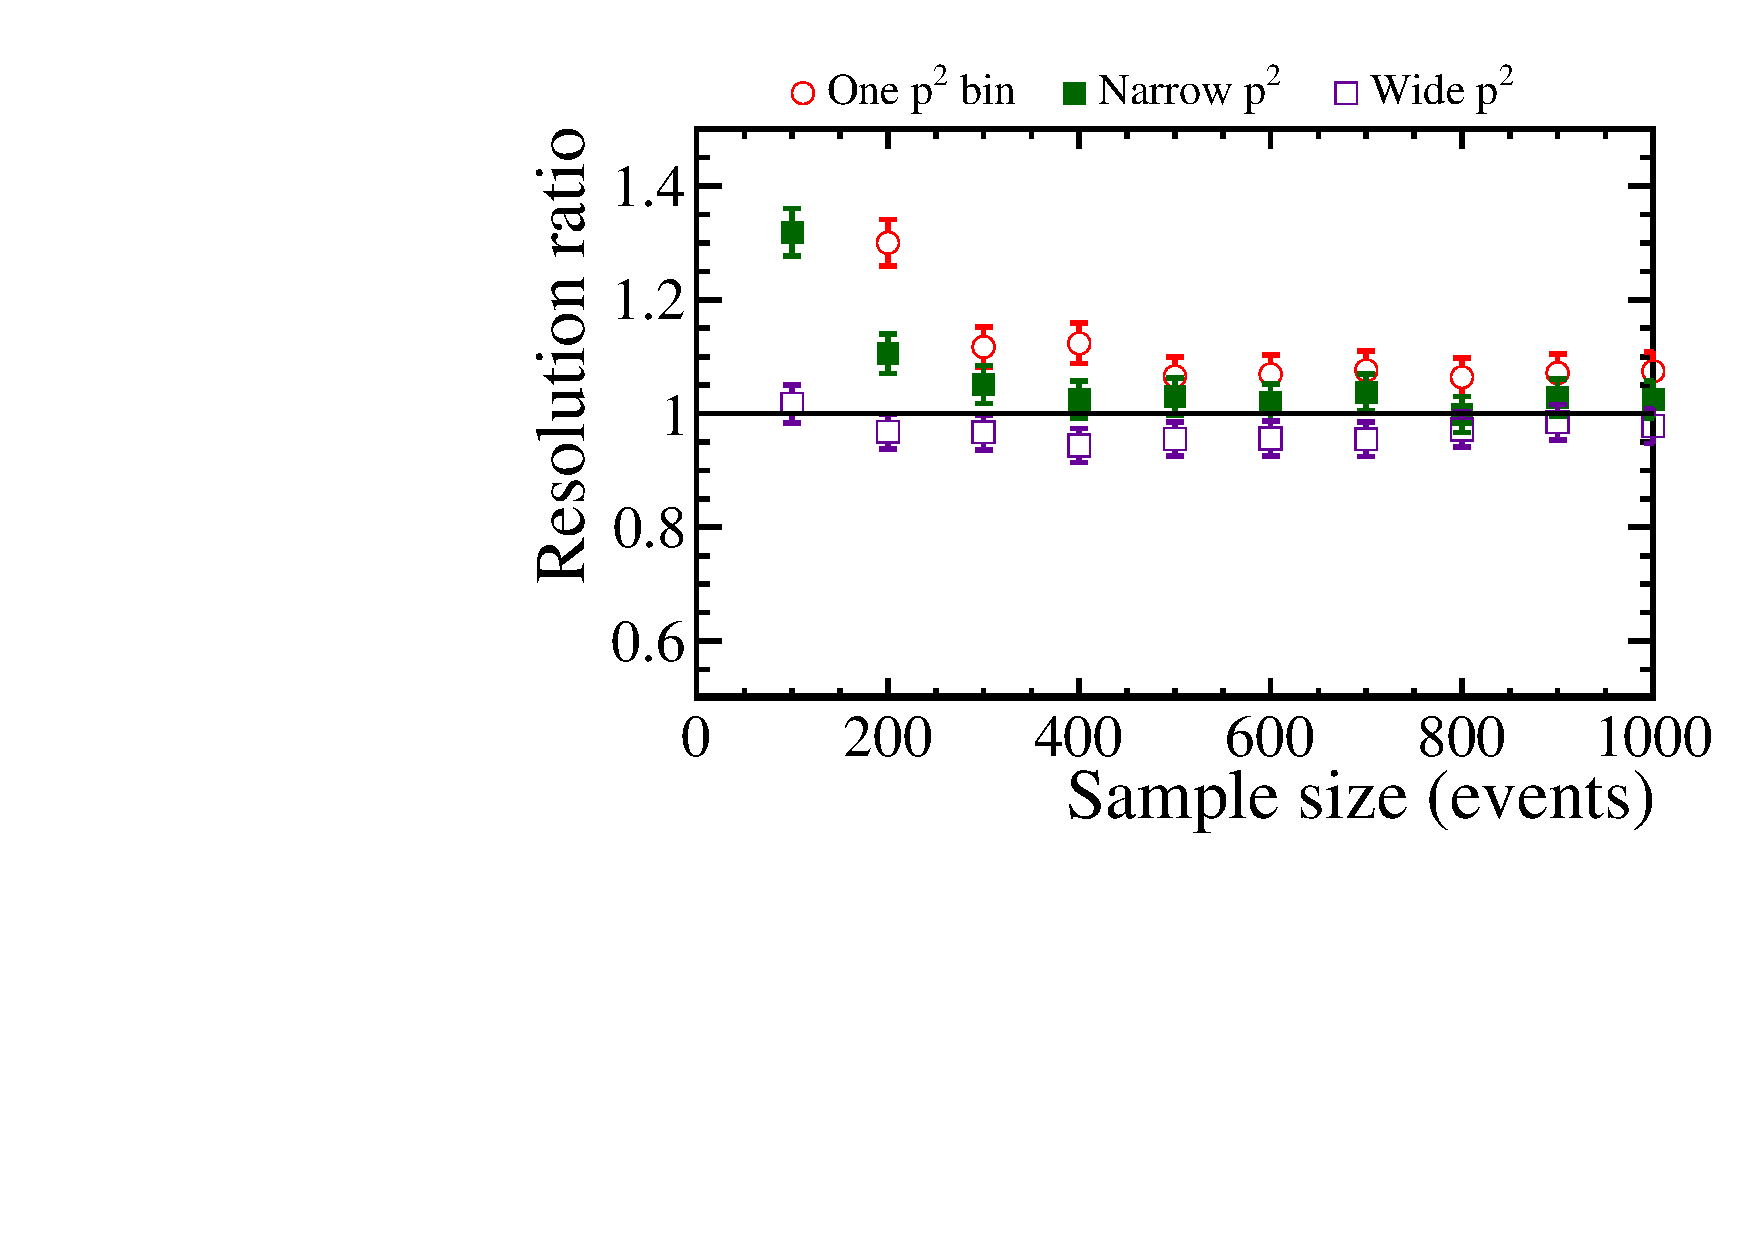
\includegraphics[width=0.48\textwidth]{chapter6/figs/fit_result_ratio_ds_afb_res.pdf}}
\subfigure[\FL]{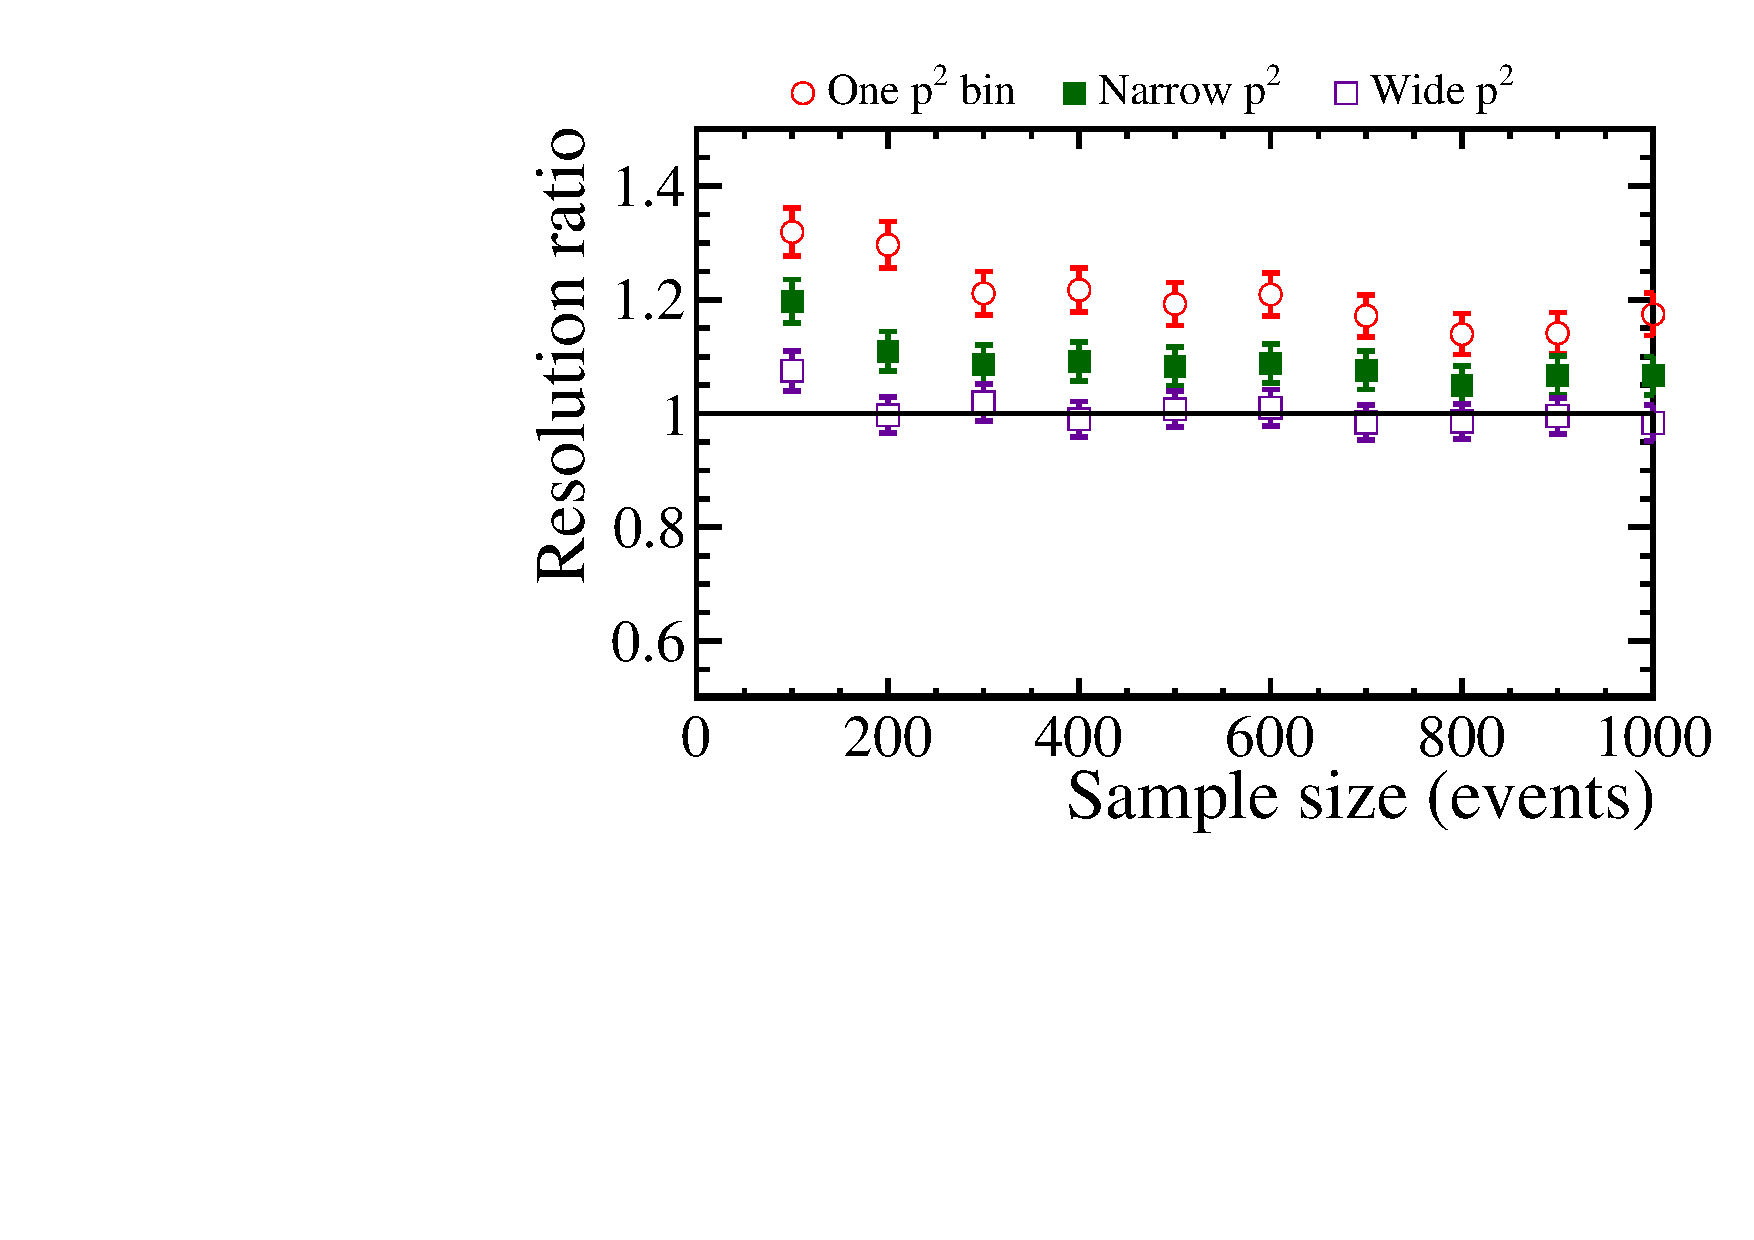
\includegraphics[width=0.48\textwidth]{chapter6/figs/fit_result_ratio_ds_fl_res.pdf}}
\subfigure[\AT2 ]{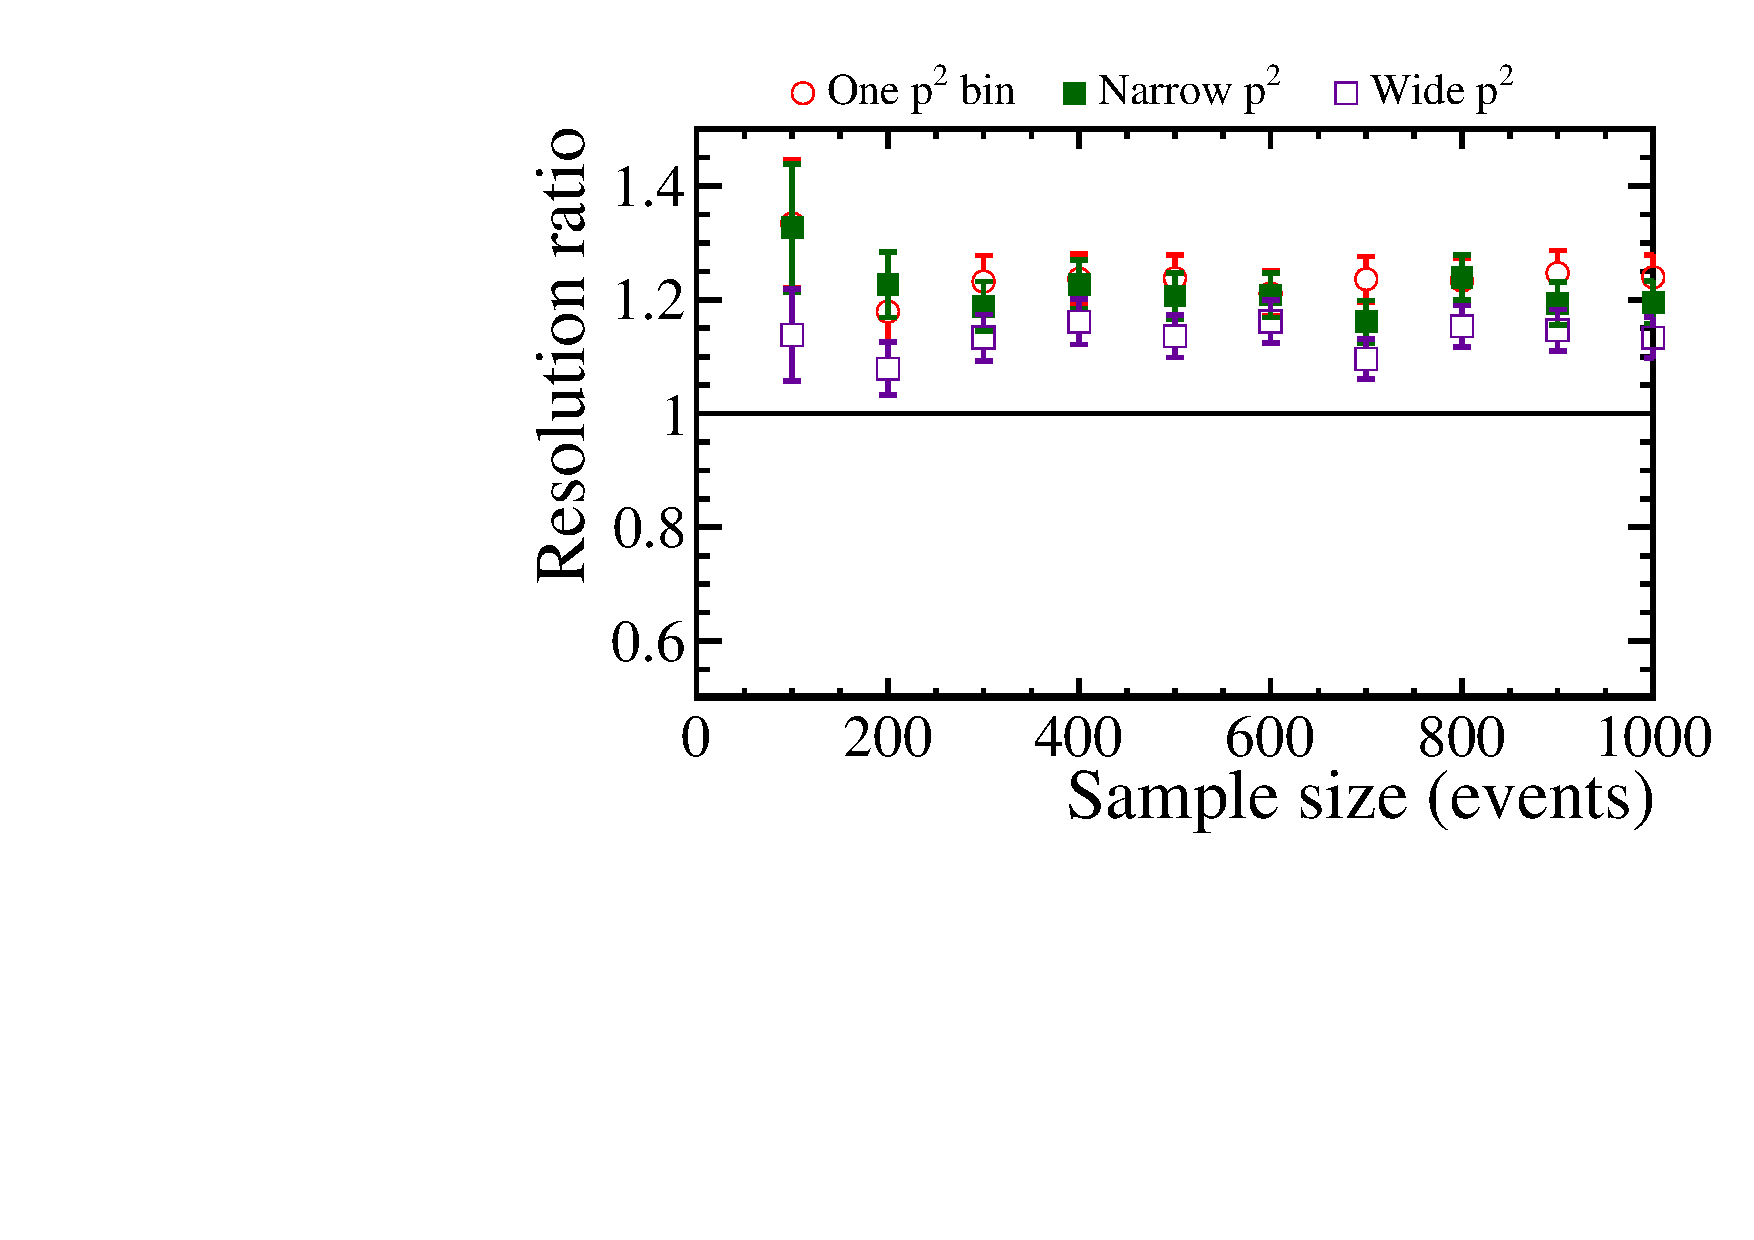
\includegraphics[width=0.48\textwidth]{chapter6/figs/fit_result_ratio_ds_at2_res.pdf}}
\subfigure[\AIm]{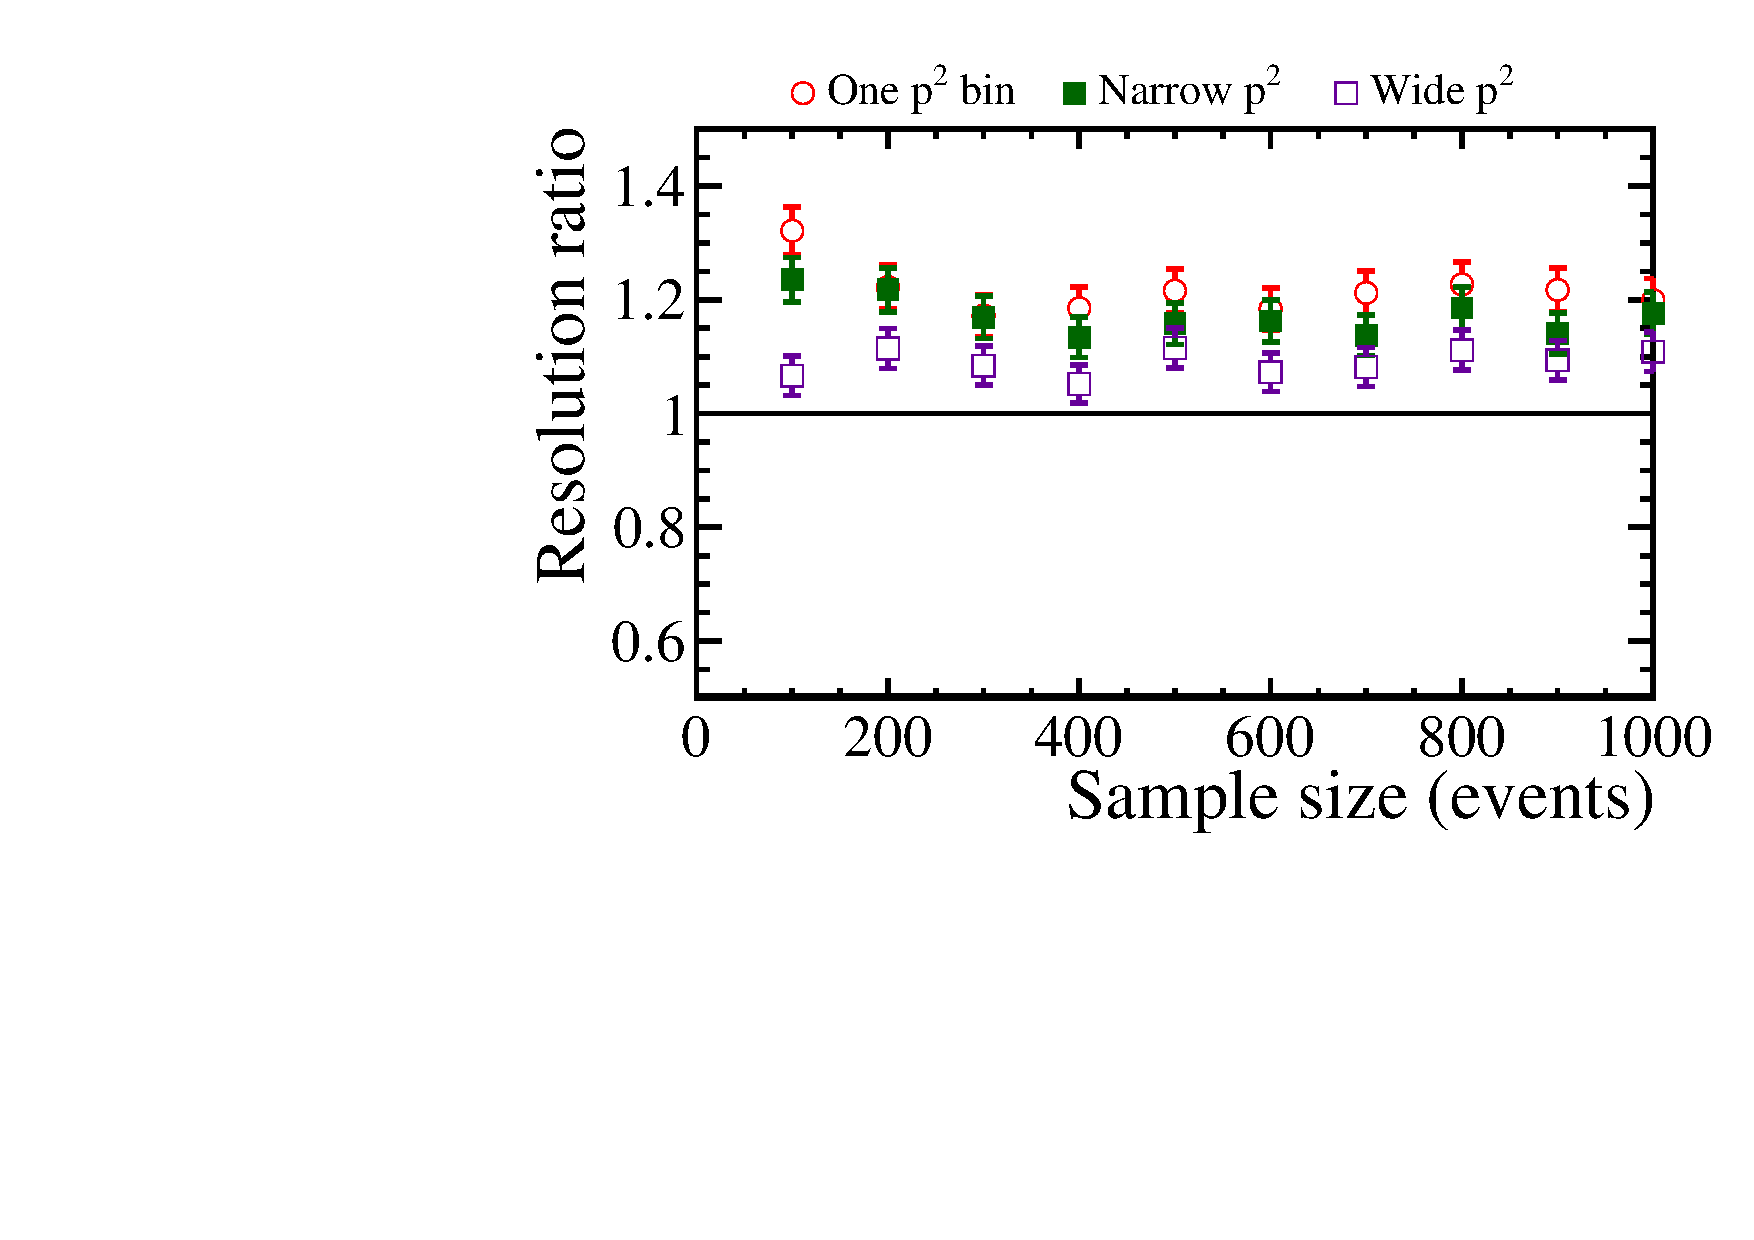
\includegraphics[width=0.48\textwidth]{chapter6/figs/fit_result_ratio_ds_aim_res.pdf}}
\caption[ Resolutions for three different methods to incorporate 
the S-wave relative to the resolution obtained when the S-wave is ignored.    ]
{Resolutions for three different methods to incorporate 
the S-wave relative to the resolution obtained when the S-wave is ignored. 
It can be seen that the best resolution is obtained when using the largest \psq window.
The original resolution is recovered to within 10\%. ~\label{fig:ratiods}}
\end{figure}
The pull mean for all three fit methods is shown in Fig~\ref{fig:combods}.
\begin{figure}[tb]
\centering
\subfigure[\AFB]{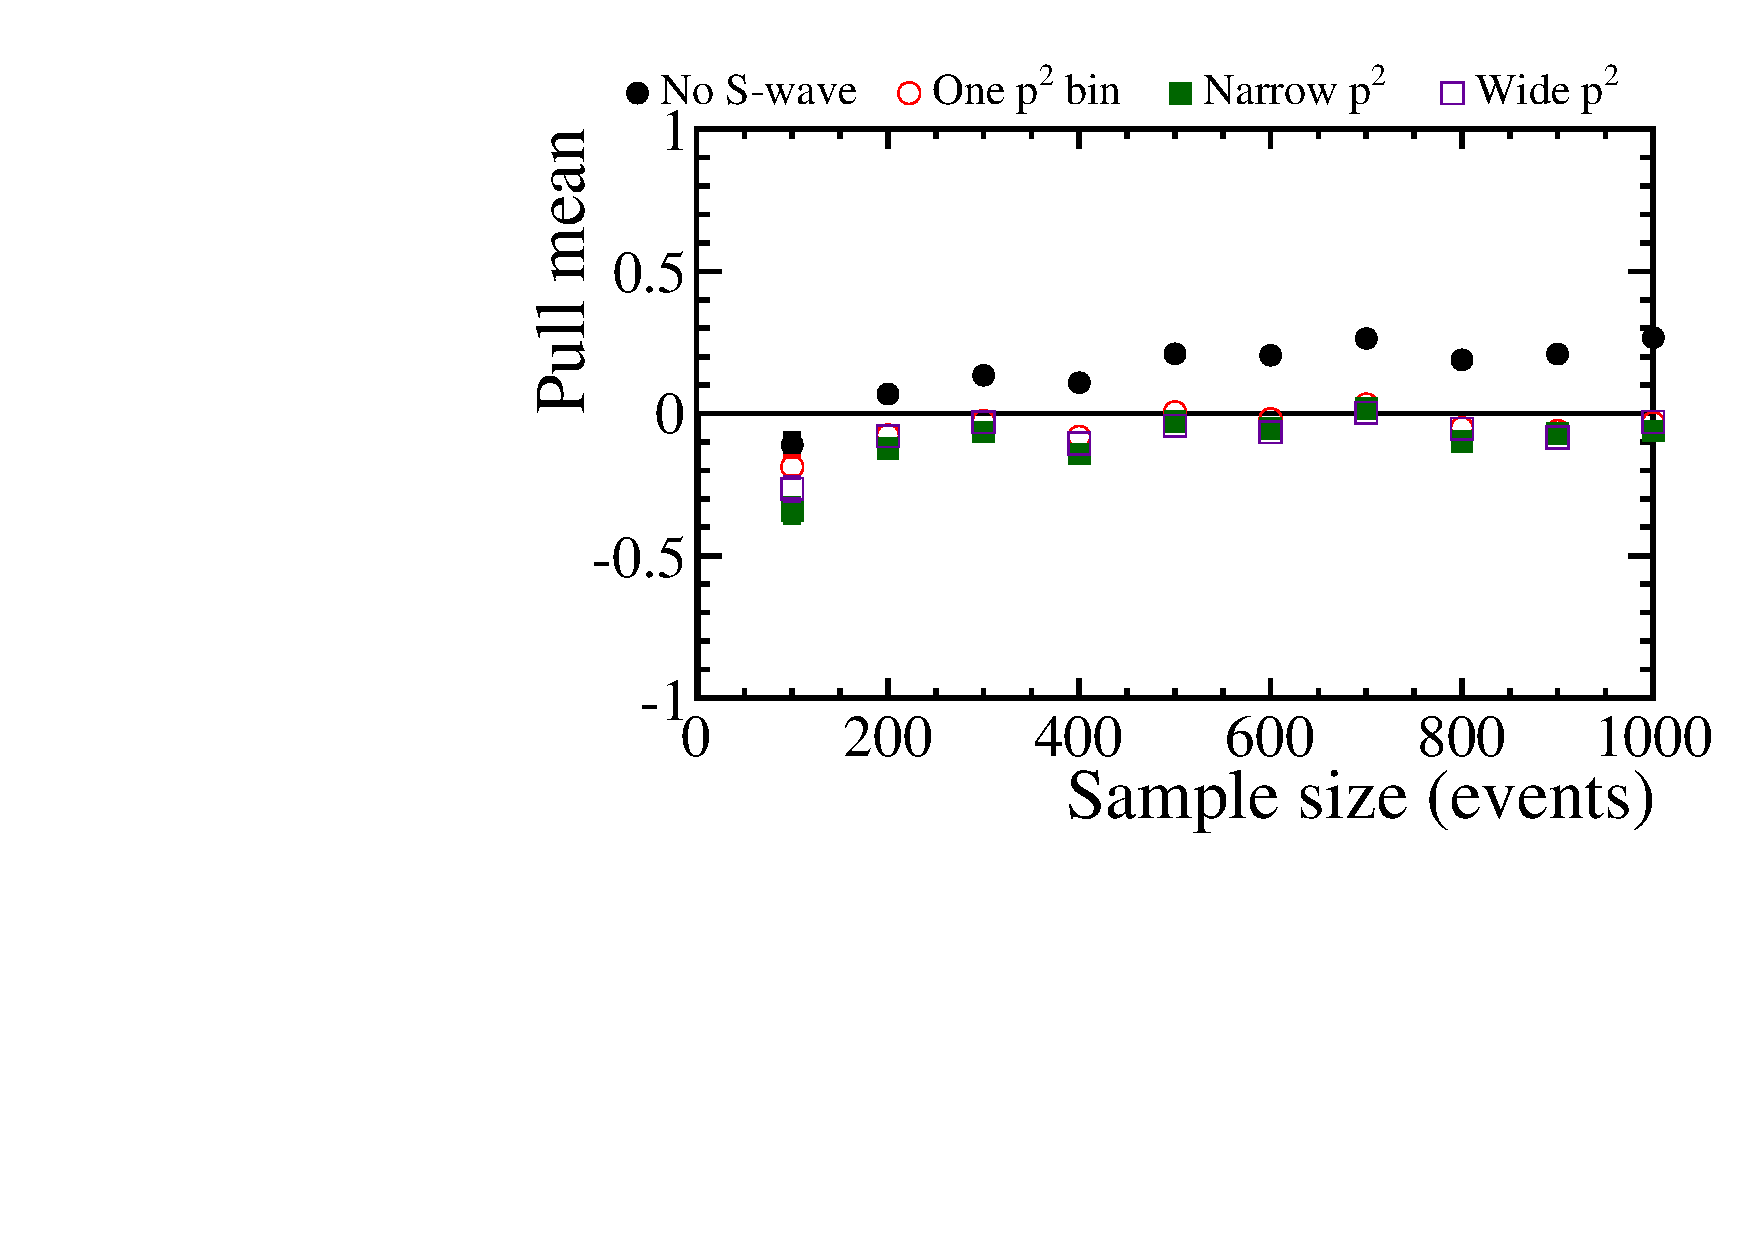
\includegraphics[width=0.48\textwidth]{chapter6/figs/fit_result_combo_ds_afb_mean.pdf}}
\subfigure[\FL]{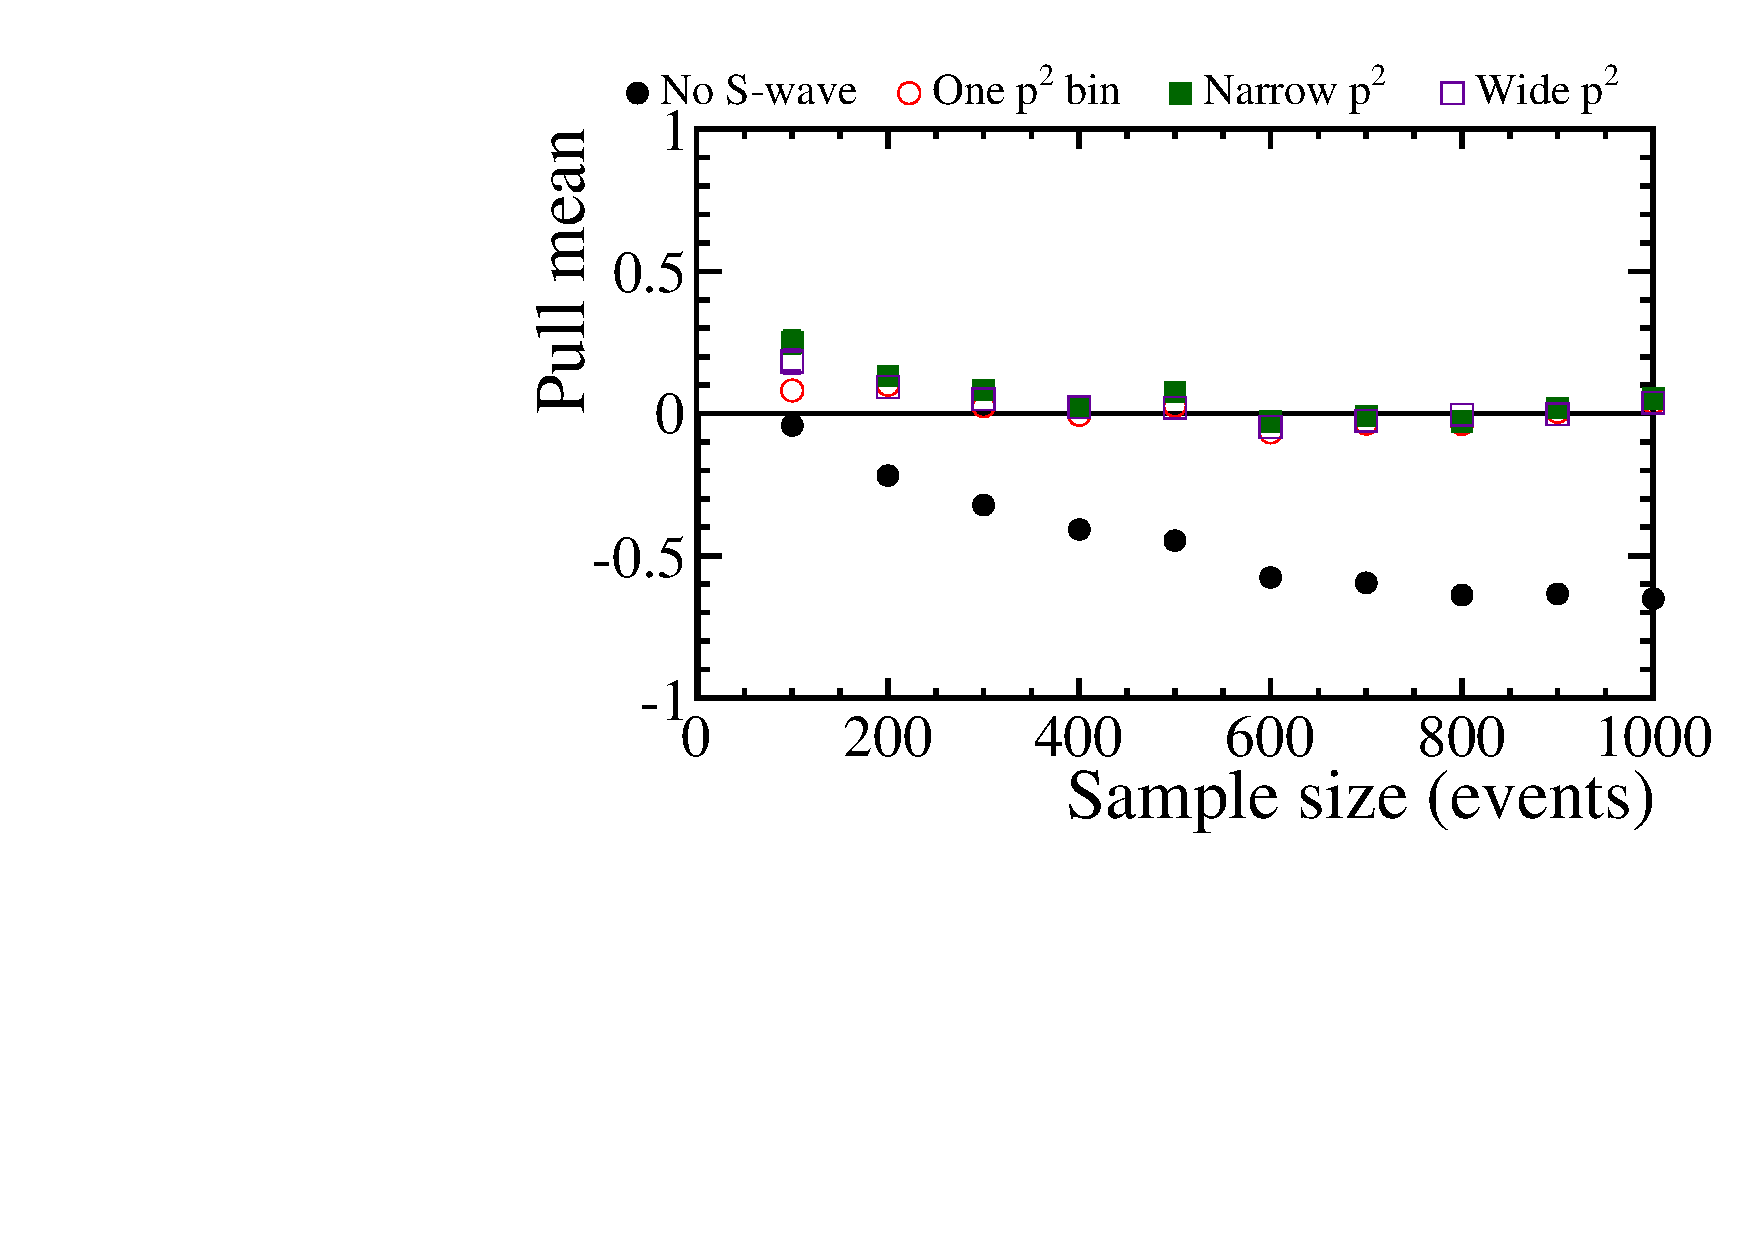
\includegraphics[width=0.48\textwidth]{chapter6/figs/fit_result_combo_ds_fl_mean.pdf}}
\subfigure[\AT2 ]{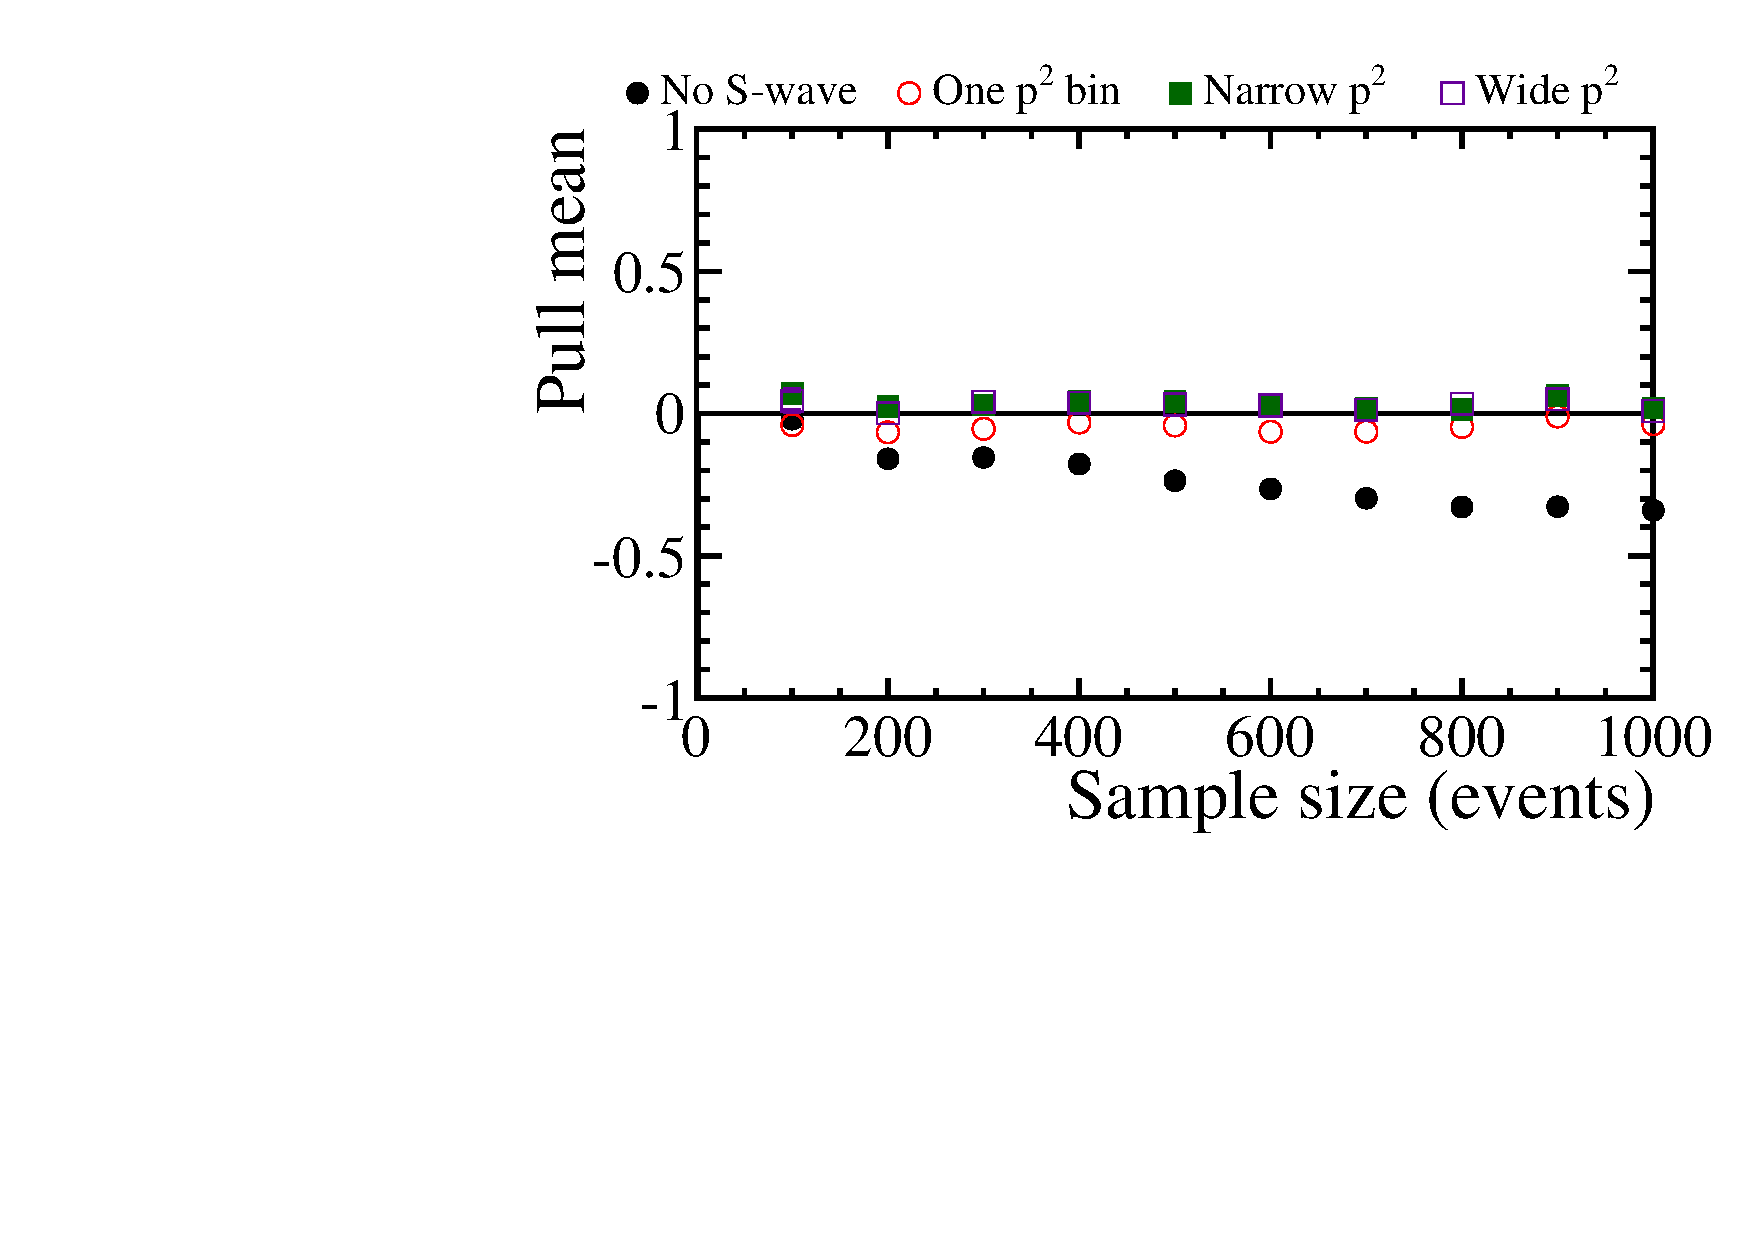
\includegraphics[width=0.48\textwidth]{chapter6/figs/fit_result_combo_ds_at2_mean.pdf}}
\subfigure[\AIm]{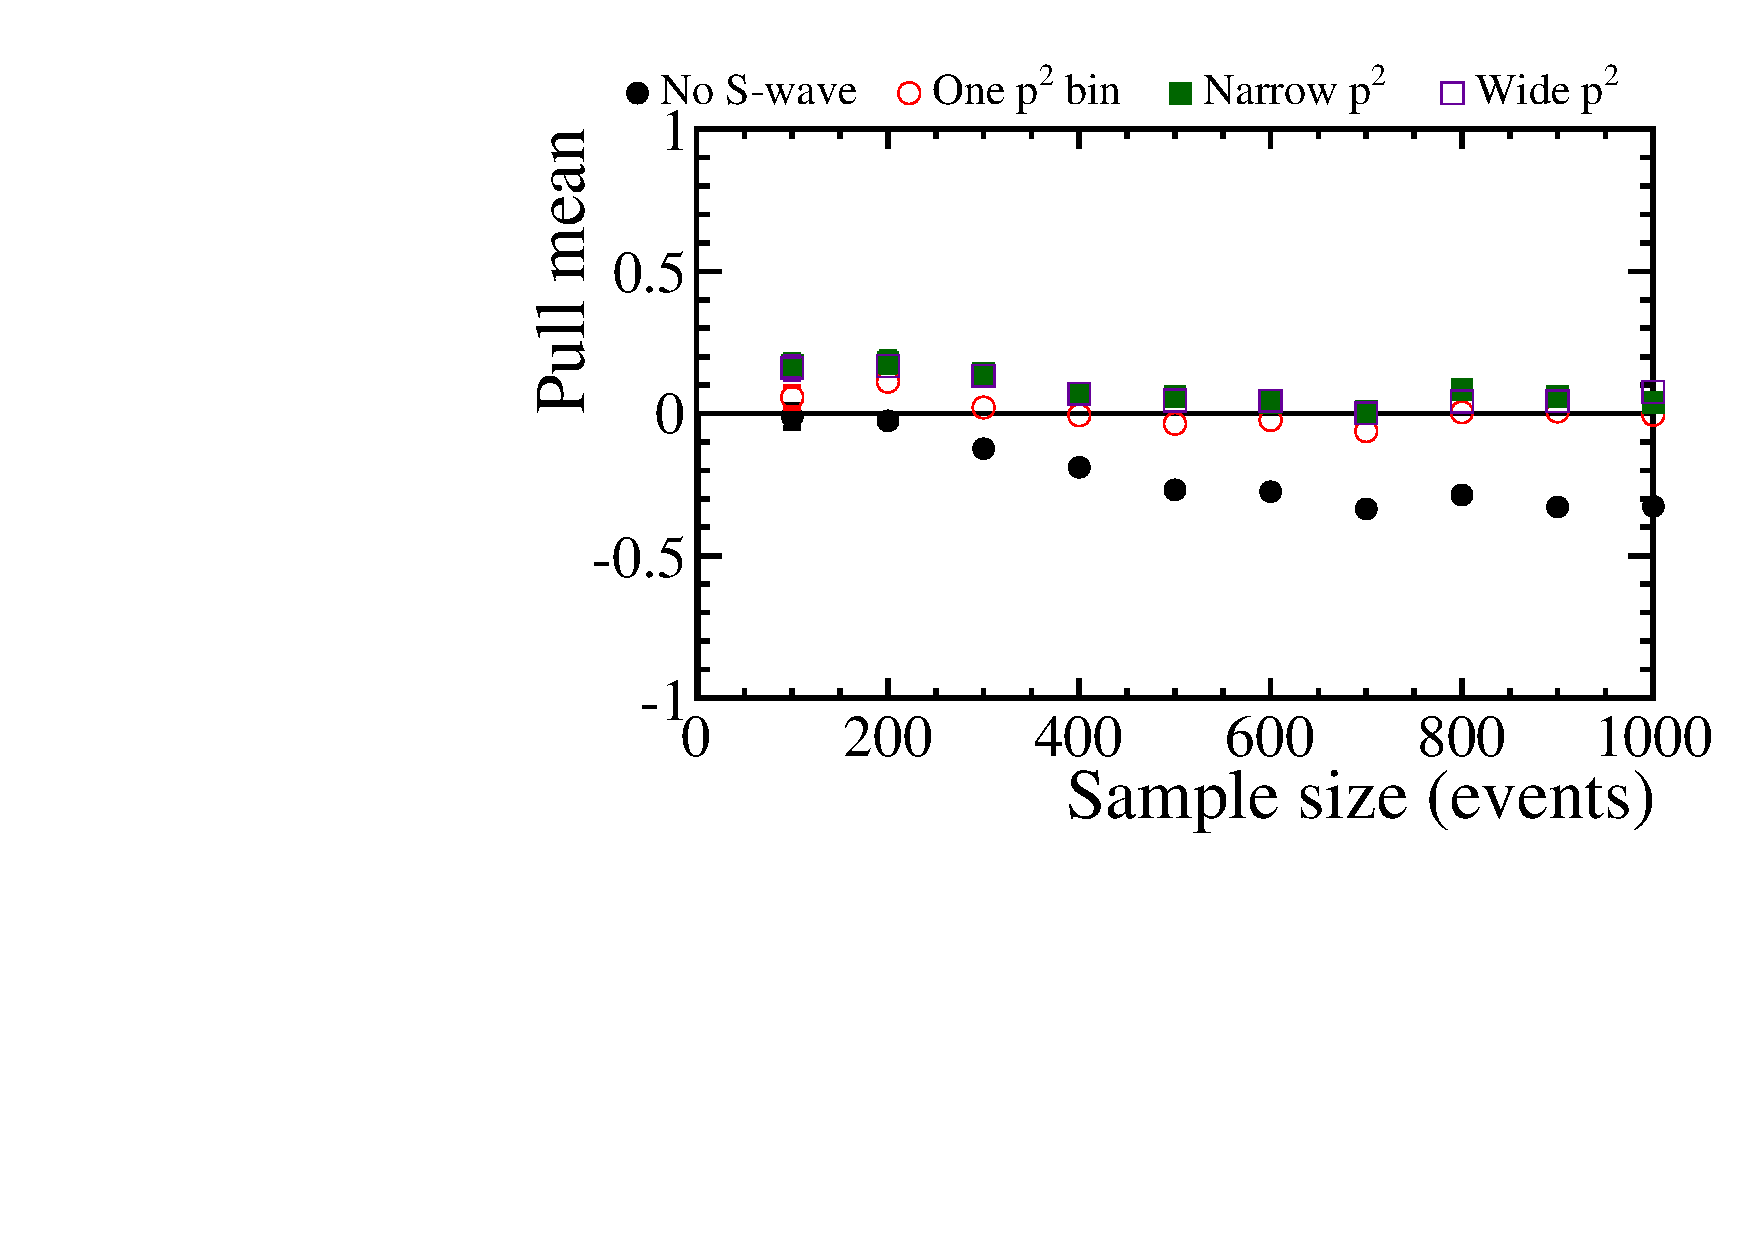
\includegraphics[width=0.48\textwidth]{chapter6/figs/fit_result_combo_ds_aim_mean.pdf}}
\caption[ Pull mean for the three different  
methods to incorporate the S-wave and when the S-wave 
is ignored.      ]
{Pull mean for the three different  
methods to incorporate the S-wave and when the S-wave 
is ignored. There is a slight shift when the S-wave is 
included for datasets of less than 200 events but this is removed from  all the observables 
when the S-wave is included in the fit 
for datasets of over 500 events. ~\label{fig:combods}}
\end{figure}
The pull width for all three fit methods is shown in Fig~\ref{fig:combodswidth}.
\begin{figure}[tb]
\centering
\subfigure[\AFB]{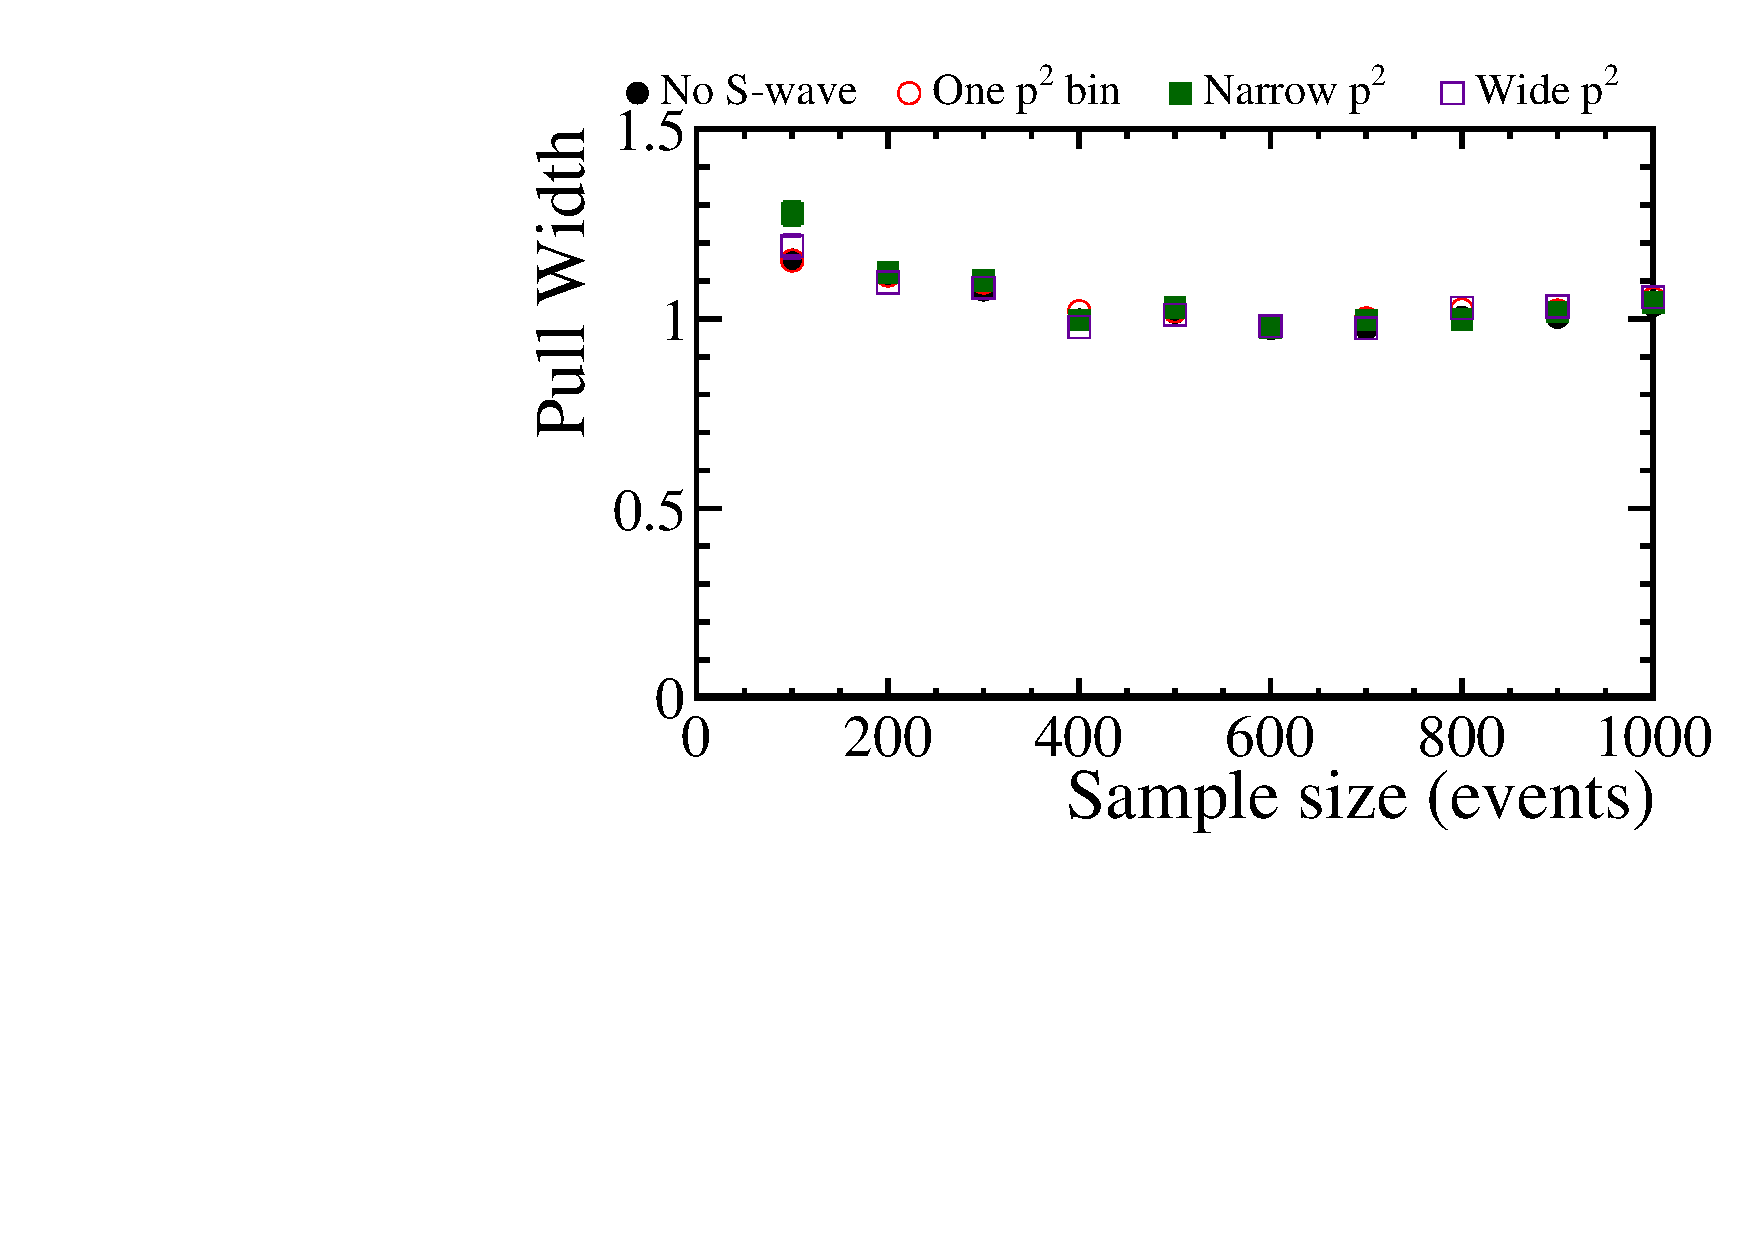
\includegraphics[width=0.48\textwidth]{chapter6/figs/fit_result_combo_ds_afb_width.pdf}}
\subfigure[\FL]{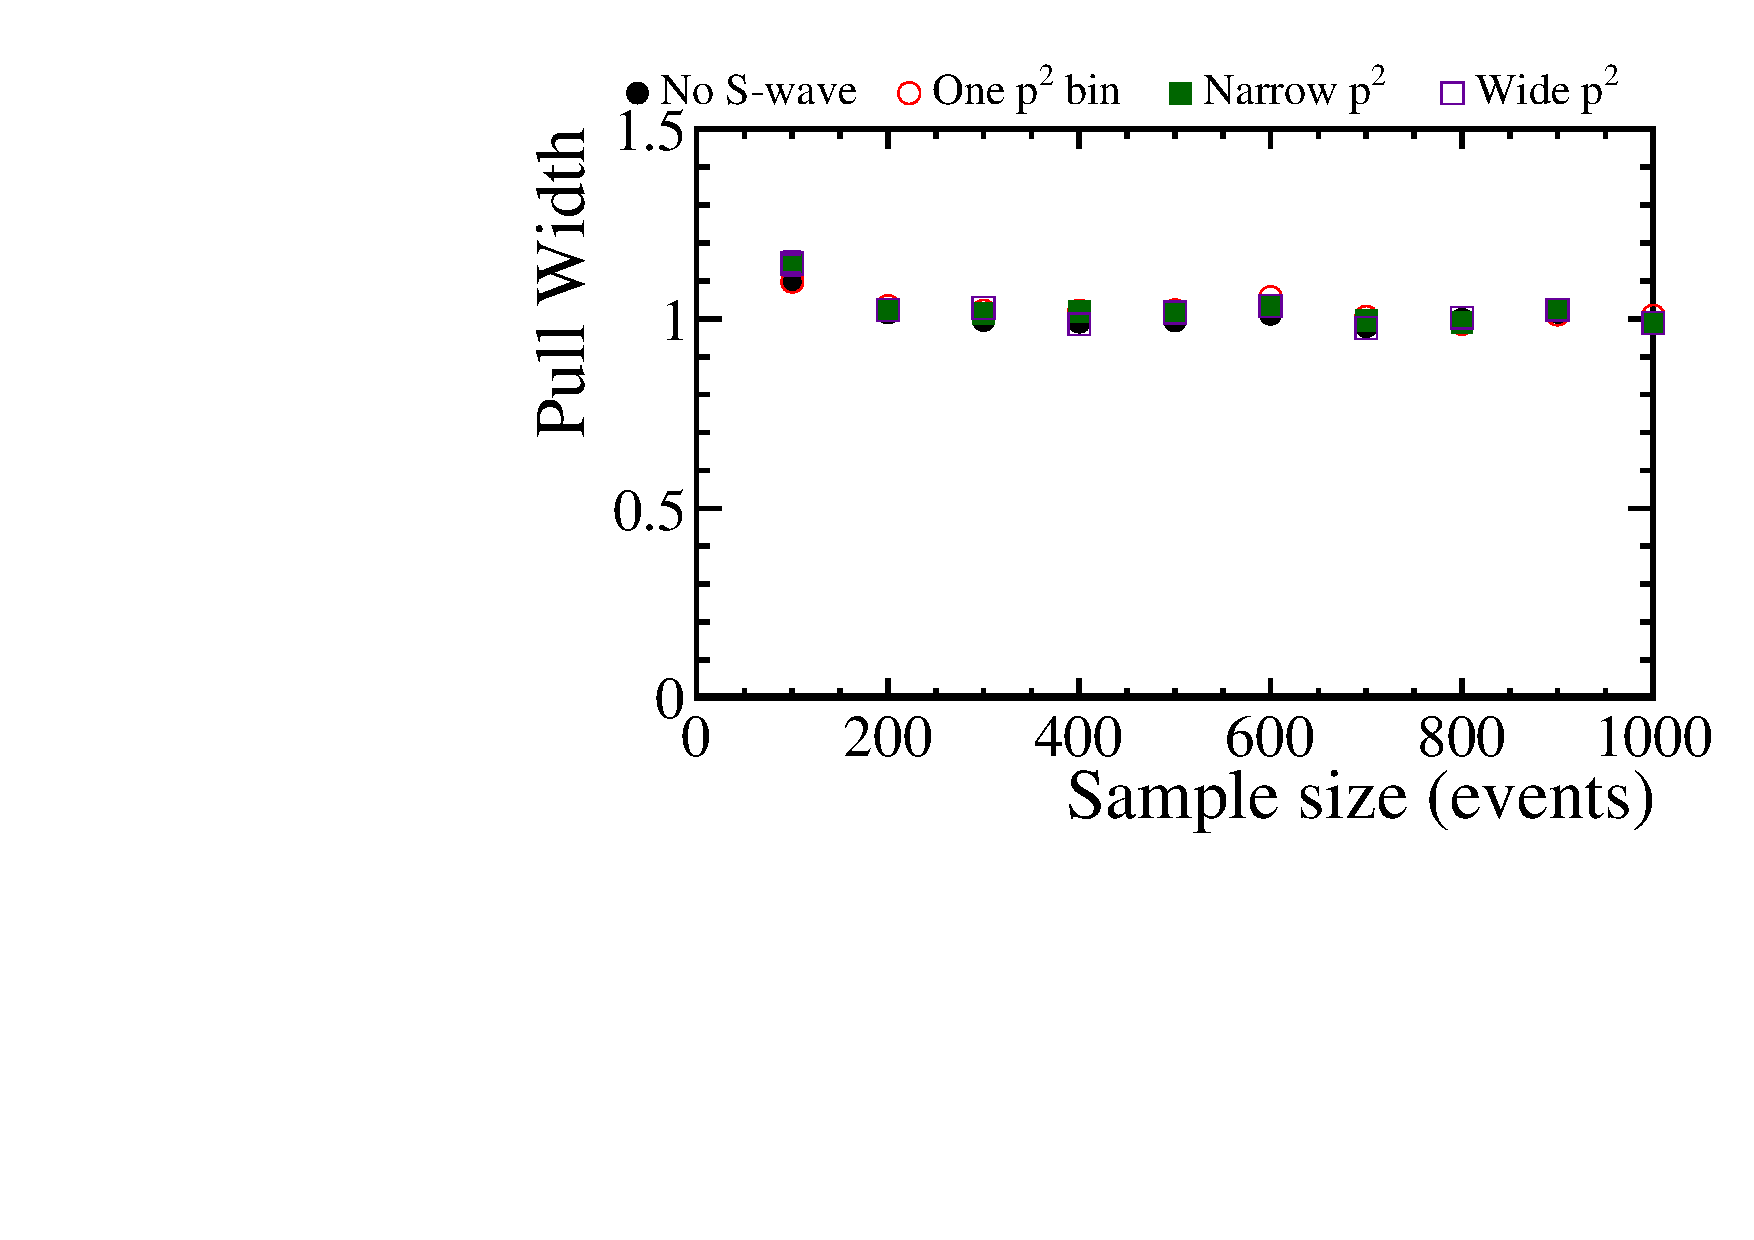
\includegraphics[width=0.48\textwidth]{chapter6/figs/fit_result_combo_ds_fl_width.pdf}}
\subfigure[\AT2 ]{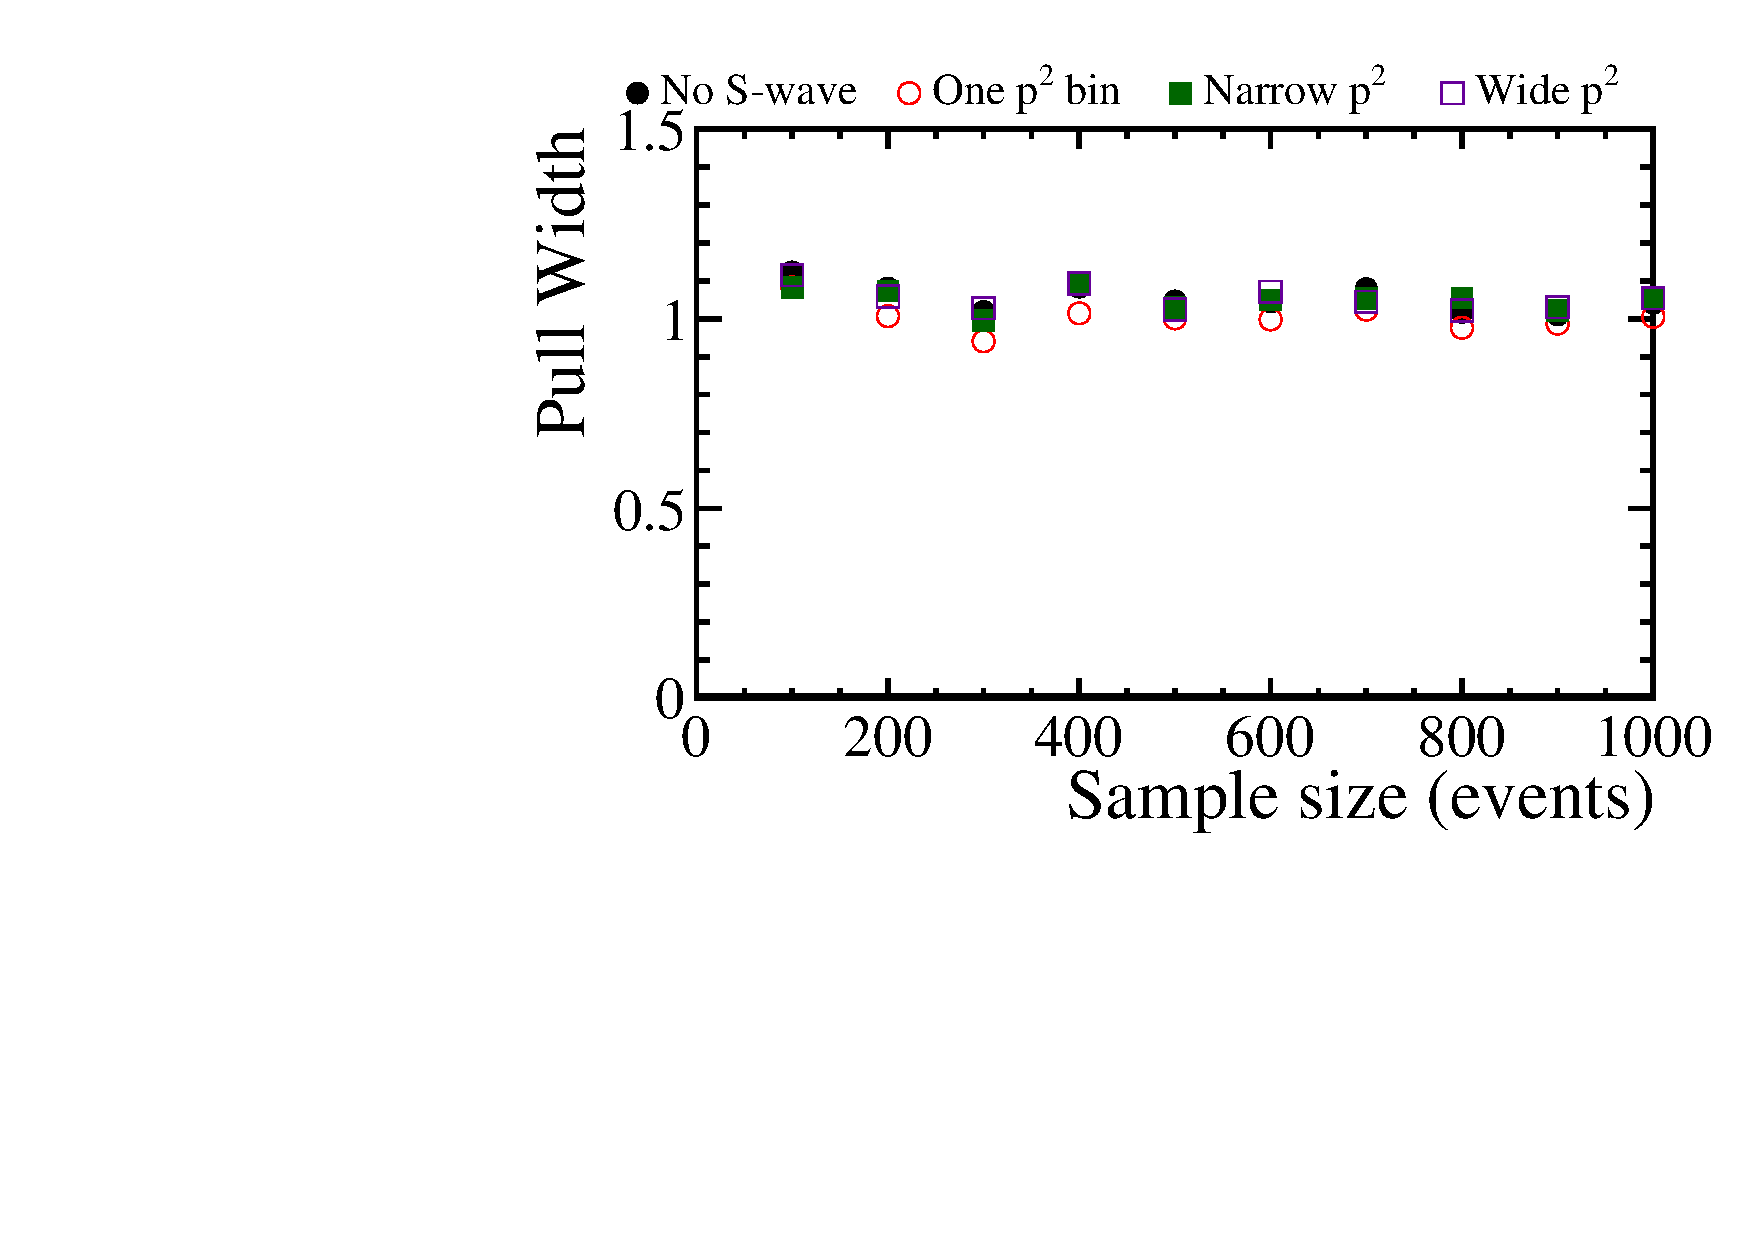
\includegraphics[width=0.48\textwidth]{chapter6/figs/fit_result_combo_ds_at2_width.pdf}}
\subfigure[\AIm]{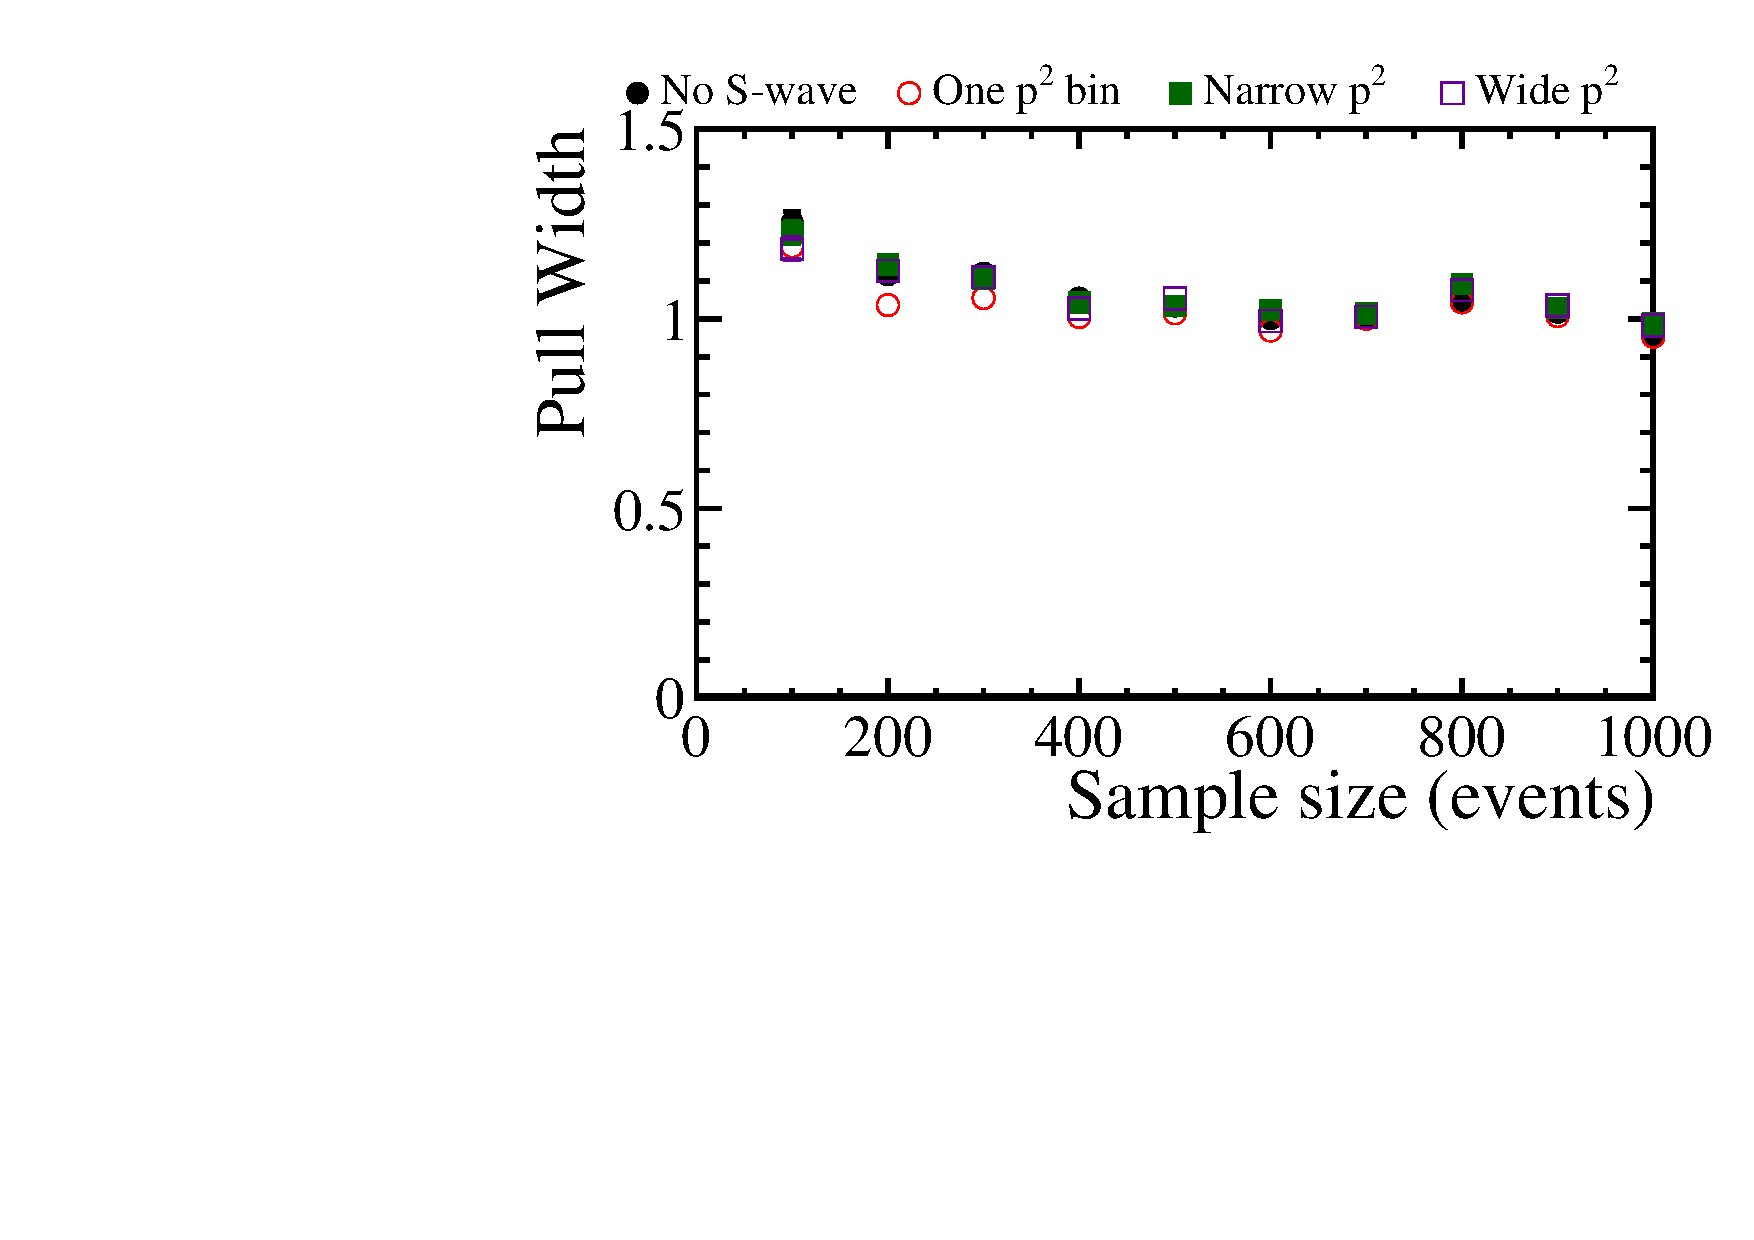
\includegraphics[width=0.48\textwidth]{chapter6/figs/fit_result_combo_ds_aim_width.pdf}}
\caption[ Pull width for the three different  
methods to incorporate the S-wave and when the S-wave 
is ignored.  ]
{Pull width for the three different  
methods to incorporate the S-wave and when the S-wave 
is ignored. There is a slight shift when the S-wave is 
included for datasets of less than 200 events but this is removed from  all the observables 
when the S-wave is included in the fit 
for datasets of over 500 events. ~\label{fig:combodswidth}}
\end{figure}

For all observables, it can be seen that the resolution degrades when
the S-wave is included and the \psq dependence is ignored.  The
resolution degrades by a smaller amount when the \psq dependence is
included in a small bin and the original resolution is recovered to
within 10\% when using the large \psq range.  There are two effects
contributing to the improvement of the resolution. There are more
P-wave events in the larger range and the wider mass window allows for
the S-wave to be constrained by using the information from above and
below the P-wave resonance.  This results in the best resolution when
the S-wave is included in the angular distribution.

For all the observables, the pull mean approaches zero for datasets of
greater than 300 events implying that the bias present in the
observables when a pure P-wave state is assumed is removed when an S-wave is
included in the angular distribution. This means that the inclusion of
the S-wave component will be mandatory for all future experimental
analyses.


The ratio of the resolutions for the three different fit methods
as a function of increasing S-wave size is given in Fig.~\ref{fig:ratiofs}.
\begin{figure}[tb]
\centering
\subfigure[\AFB]{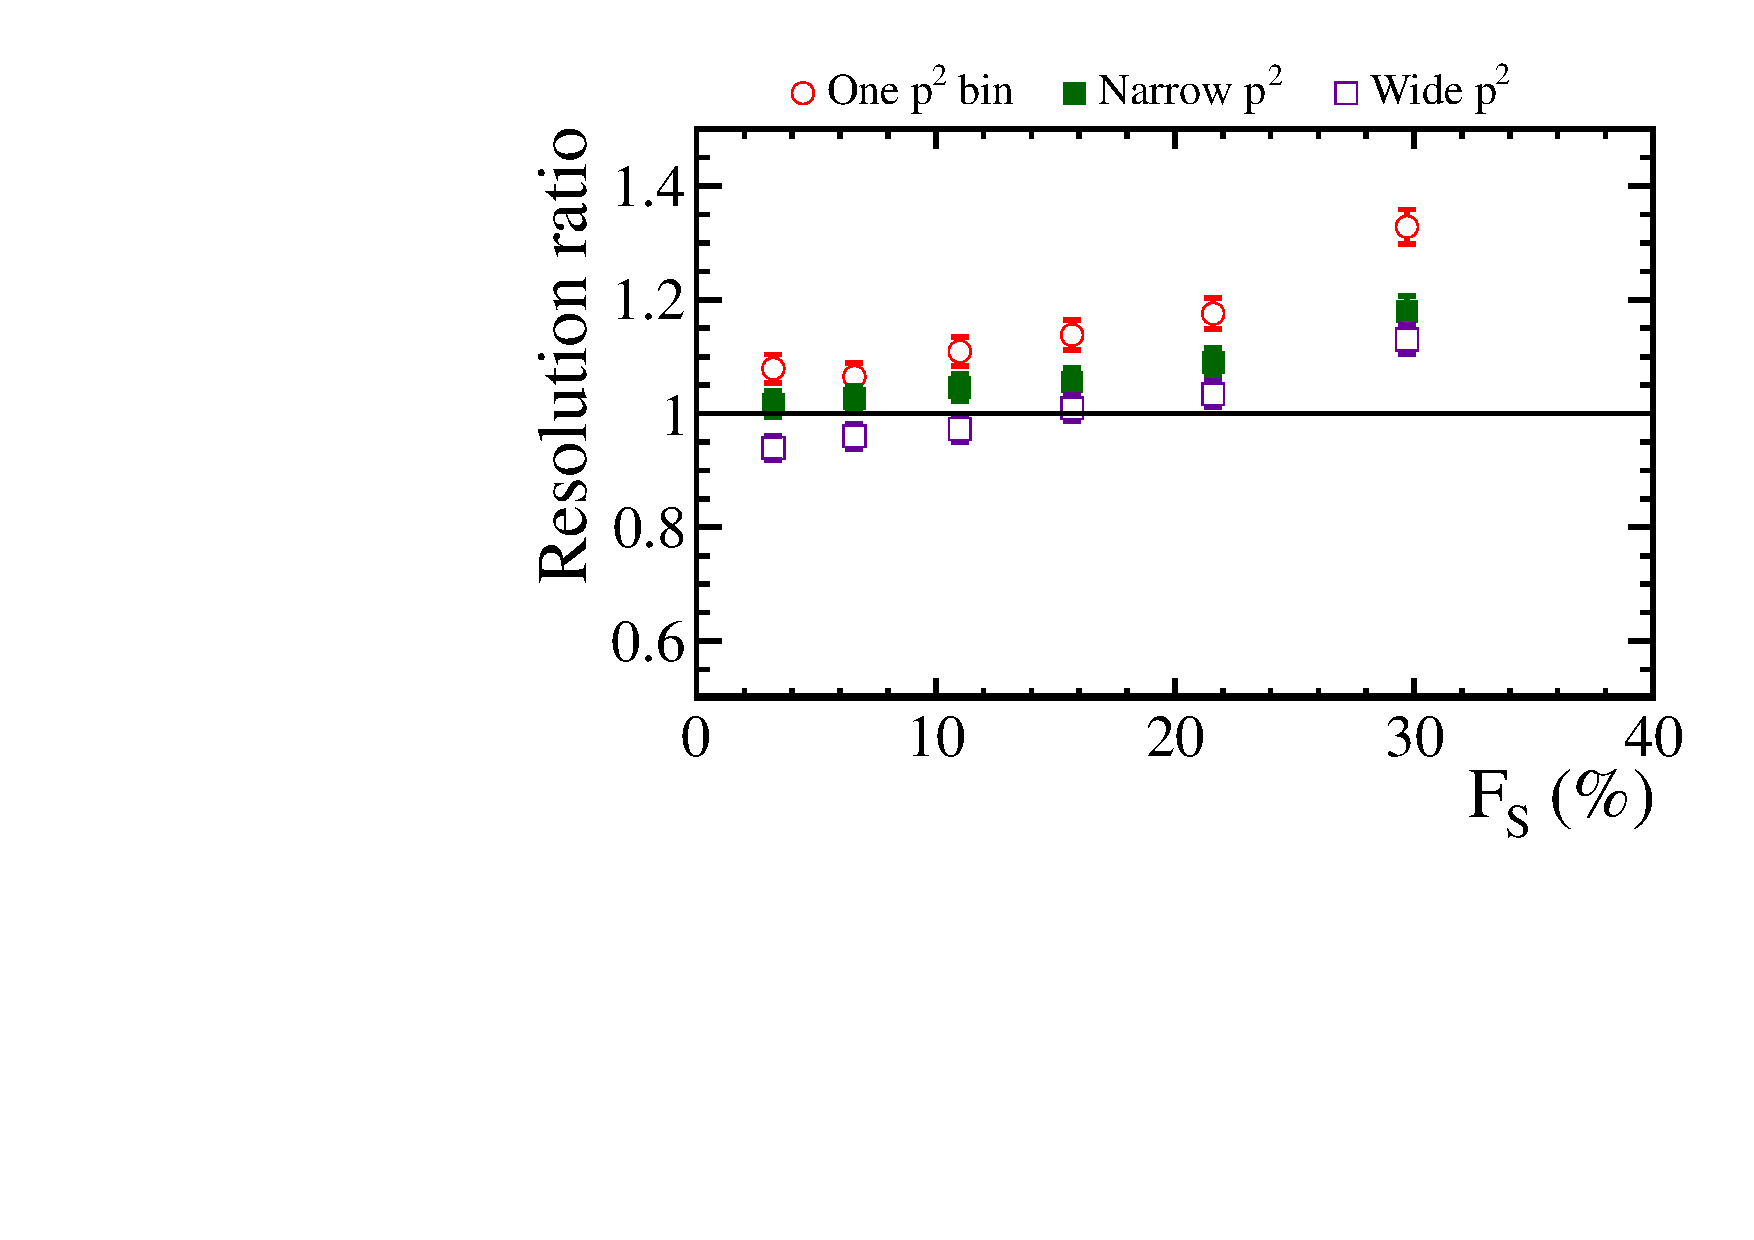
\includegraphics[width=0.48\textwidth]{chapter6/figs/fit_result_ratio_fs_afb_res.pdf}}
\subfigure[\FL]{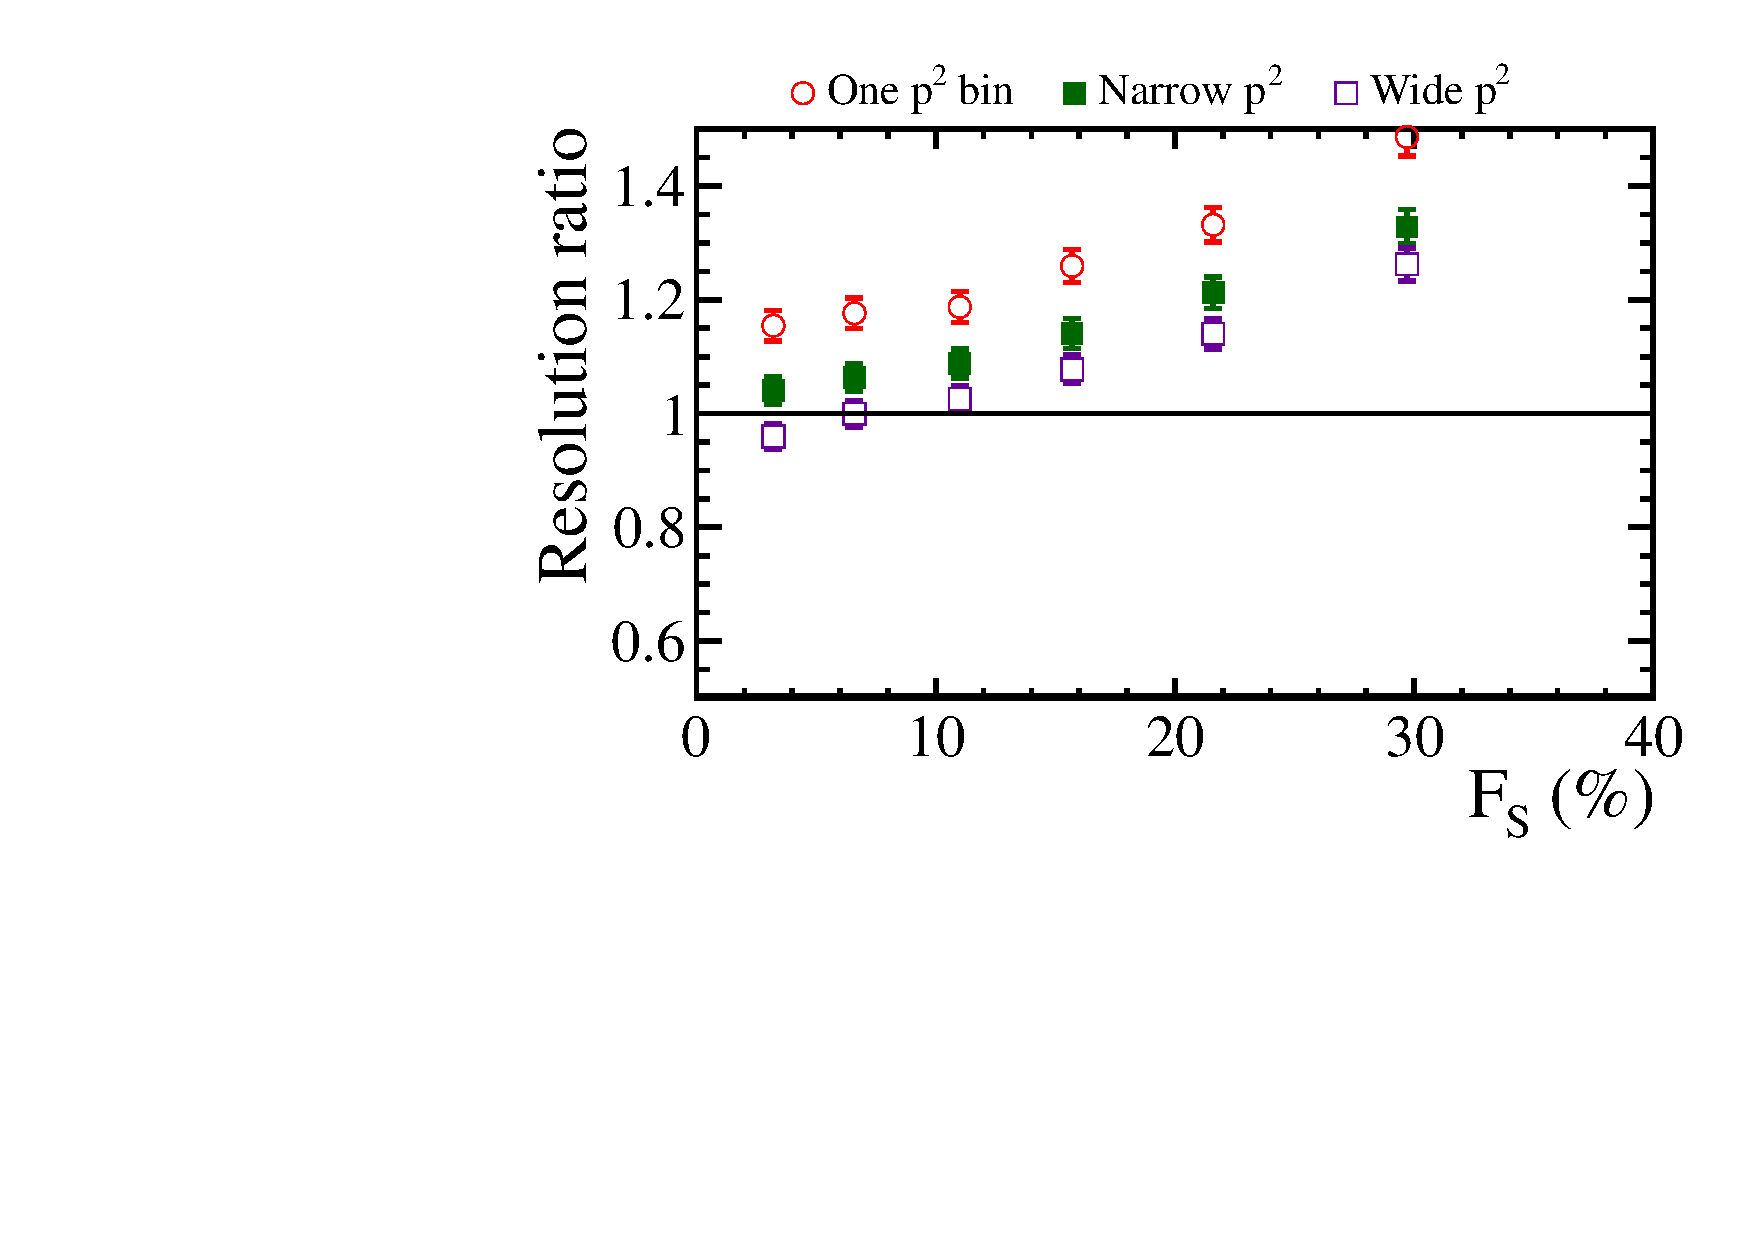
\includegraphics[width=0.48\textwidth]{chapter6/figs/fit_result_ratio_fs_fl_res.pdf}}
\subfigure[\AT2 ]{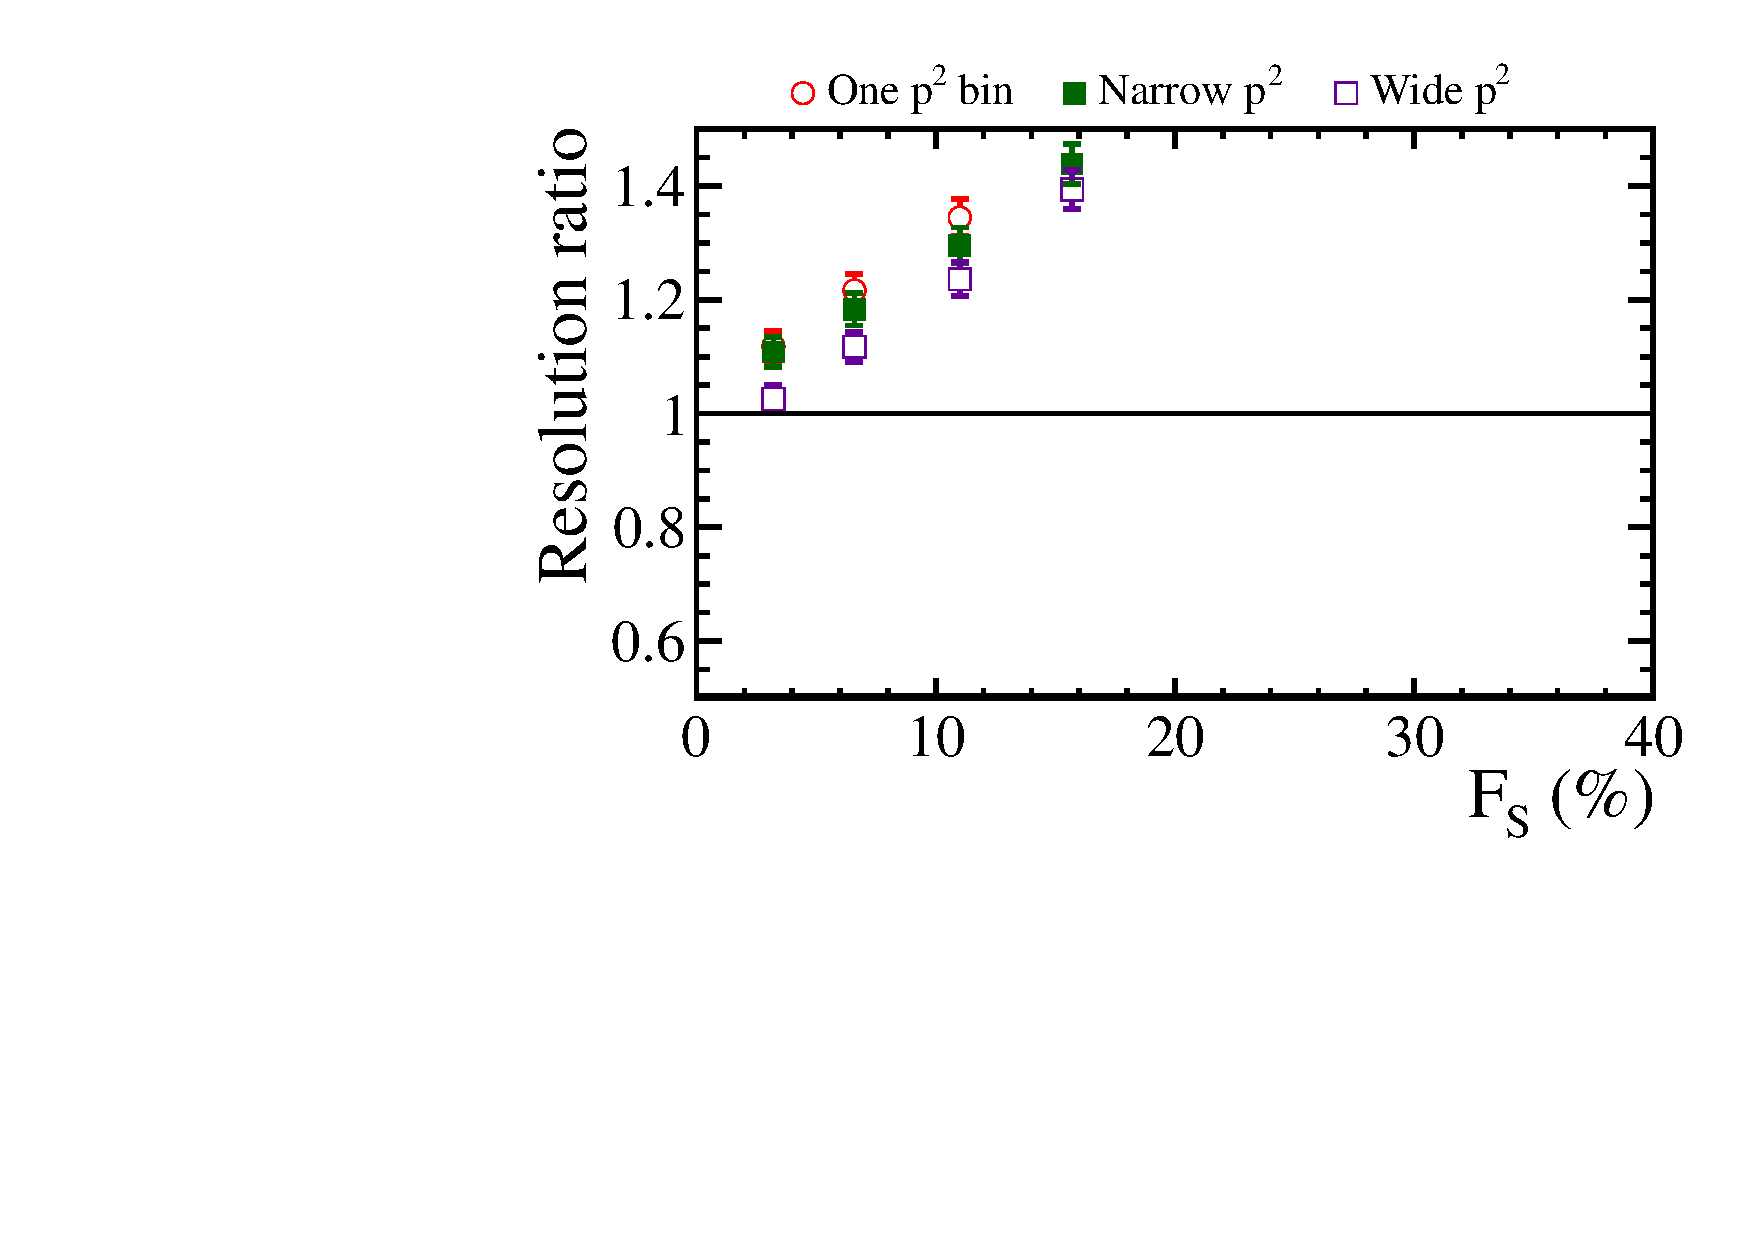
\includegraphics[width=0.48\textwidth]{chapter6/figs/fit_result_ratio_fs_at2_res.pdf}}
\subfigure[\AIm]{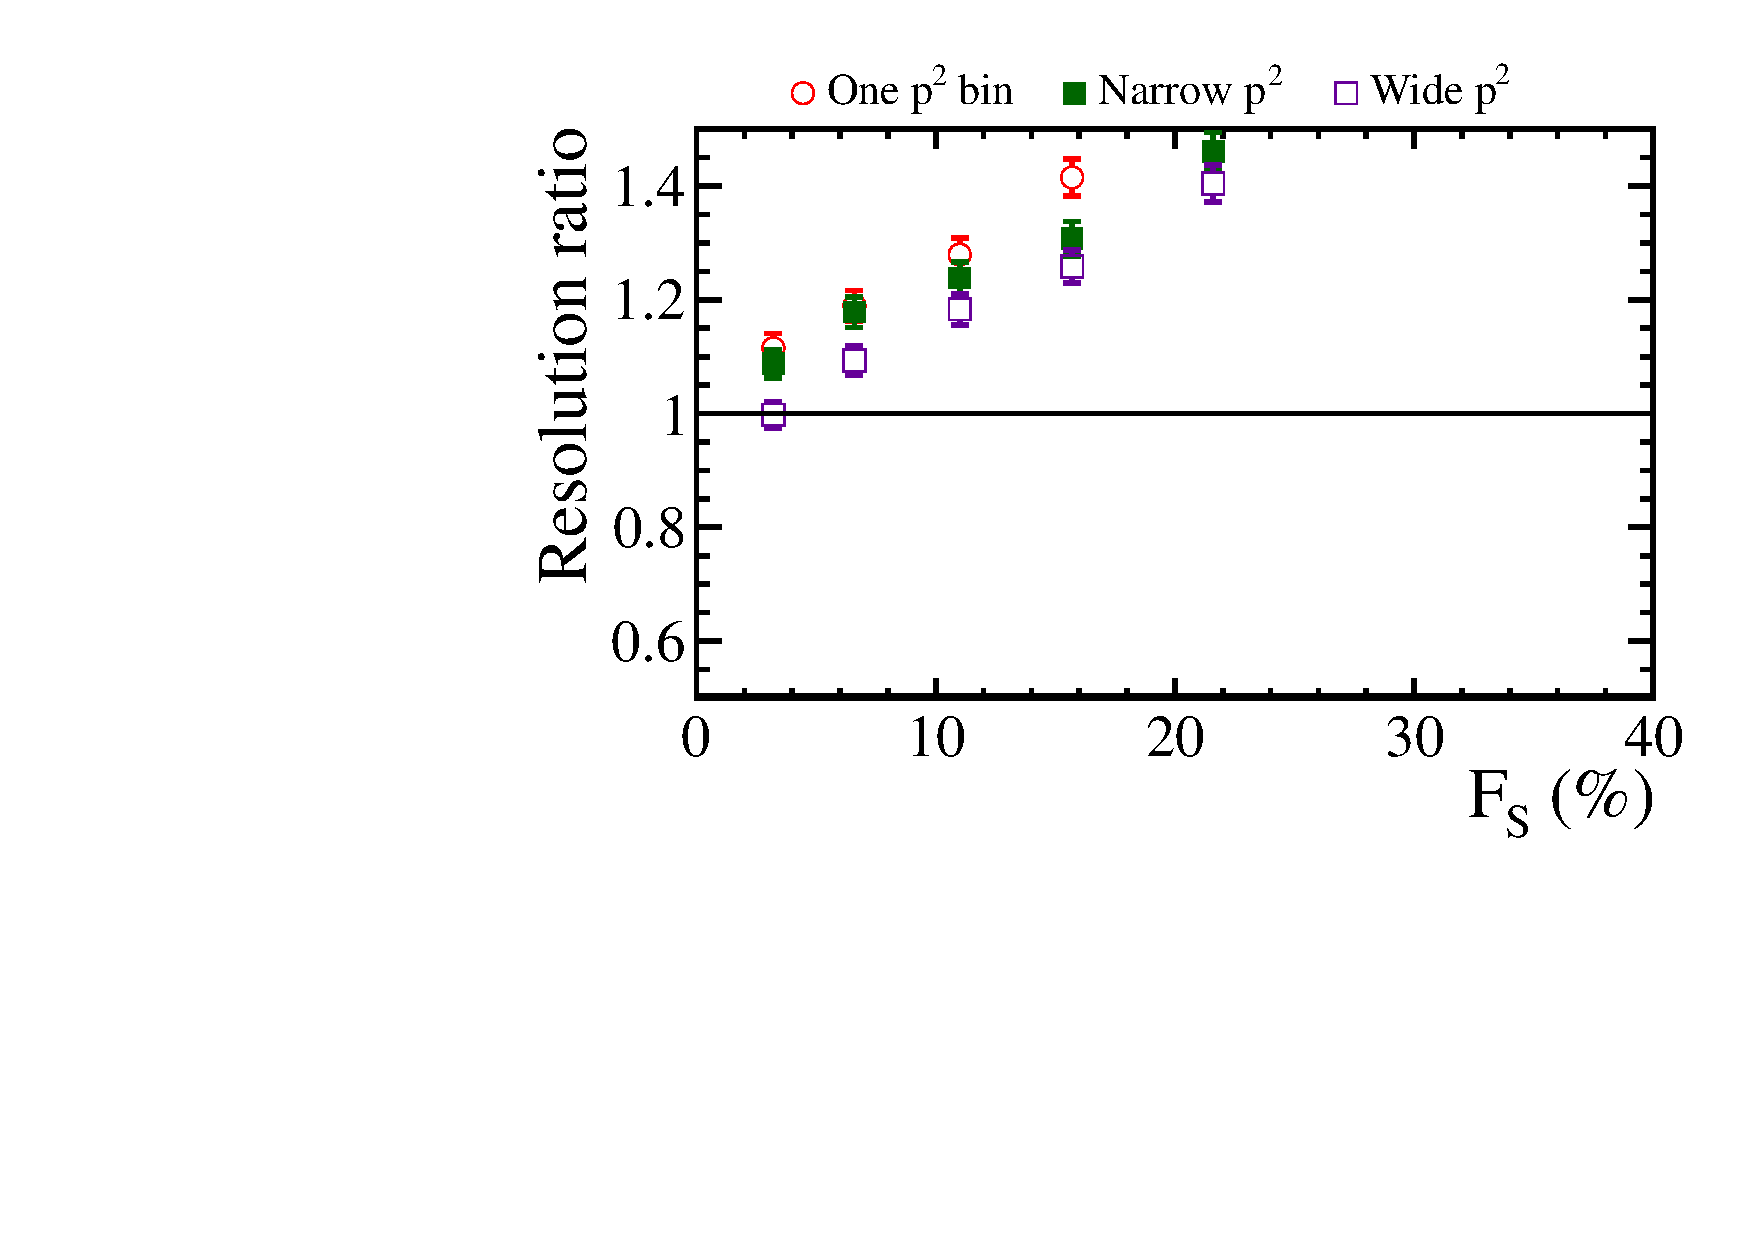
\includegraphics[width=0.48\textwidth]{chapter6/figs/fit_result_ratio_fs_aim_res.pdf}}
\caption[  Resolutions for three different methods to incorporate 
the S-wave relative to the resolution obtained when the S-wave is ignored.   ]
{Resolutions for three different methods to incorporate 
the S-wave relative to the resolution obtained when the S-wave is ignored. 
It can be seen that the best resolution is obtained when using the largest \psq window.
The original resolution is recovered to within 10\%. ~\label{fig:ratiofs}}
\end{figure}
The pull mean  as a function of S-wave contribution 
for all three fit methods is shown in Fig.~\ref{fig:combofs}.
\begin{figure}[tb]
\centering
\subfigure[\AFB]{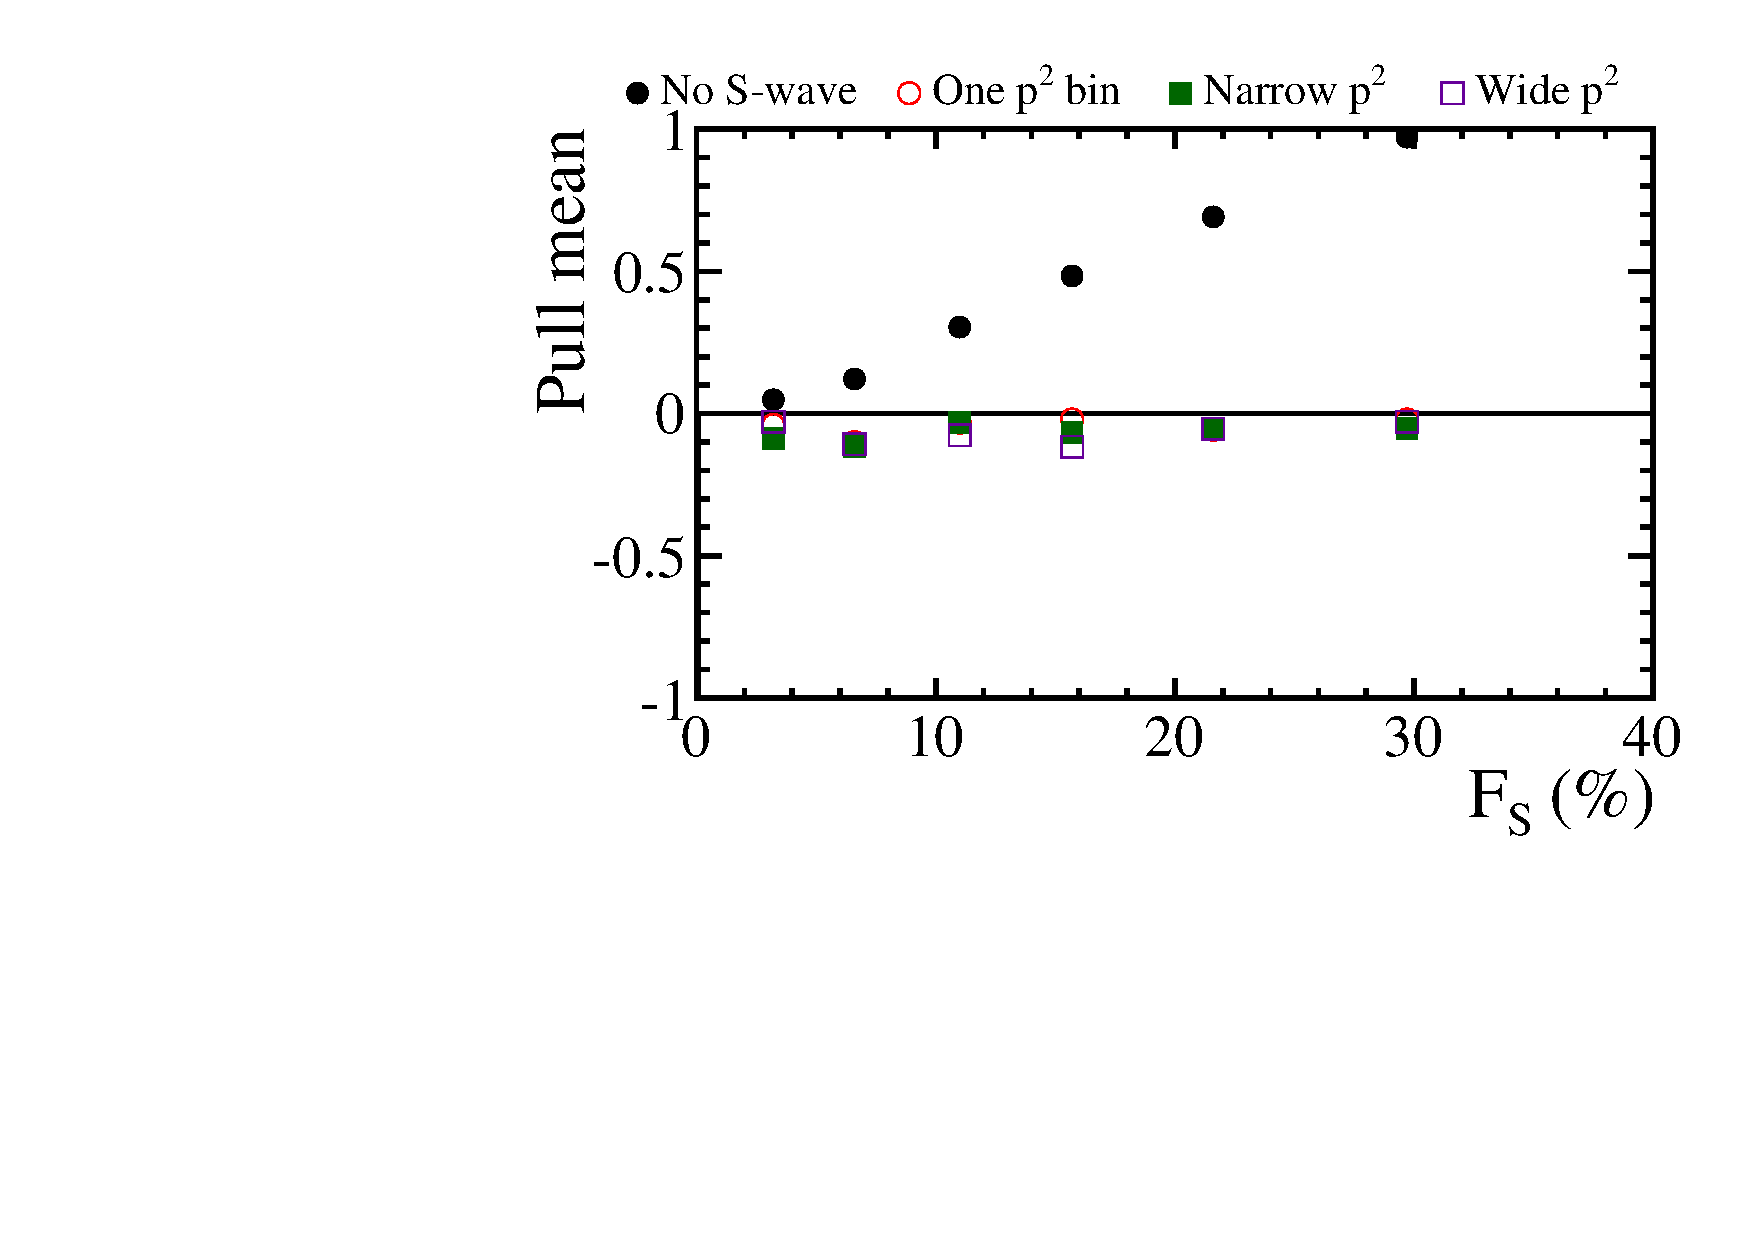
\includegraphics[width=0.48\textwidth]{chapter6/figs/fit_result_combo_fs_afb_mean.pdf}}
\subfigure[\FL]{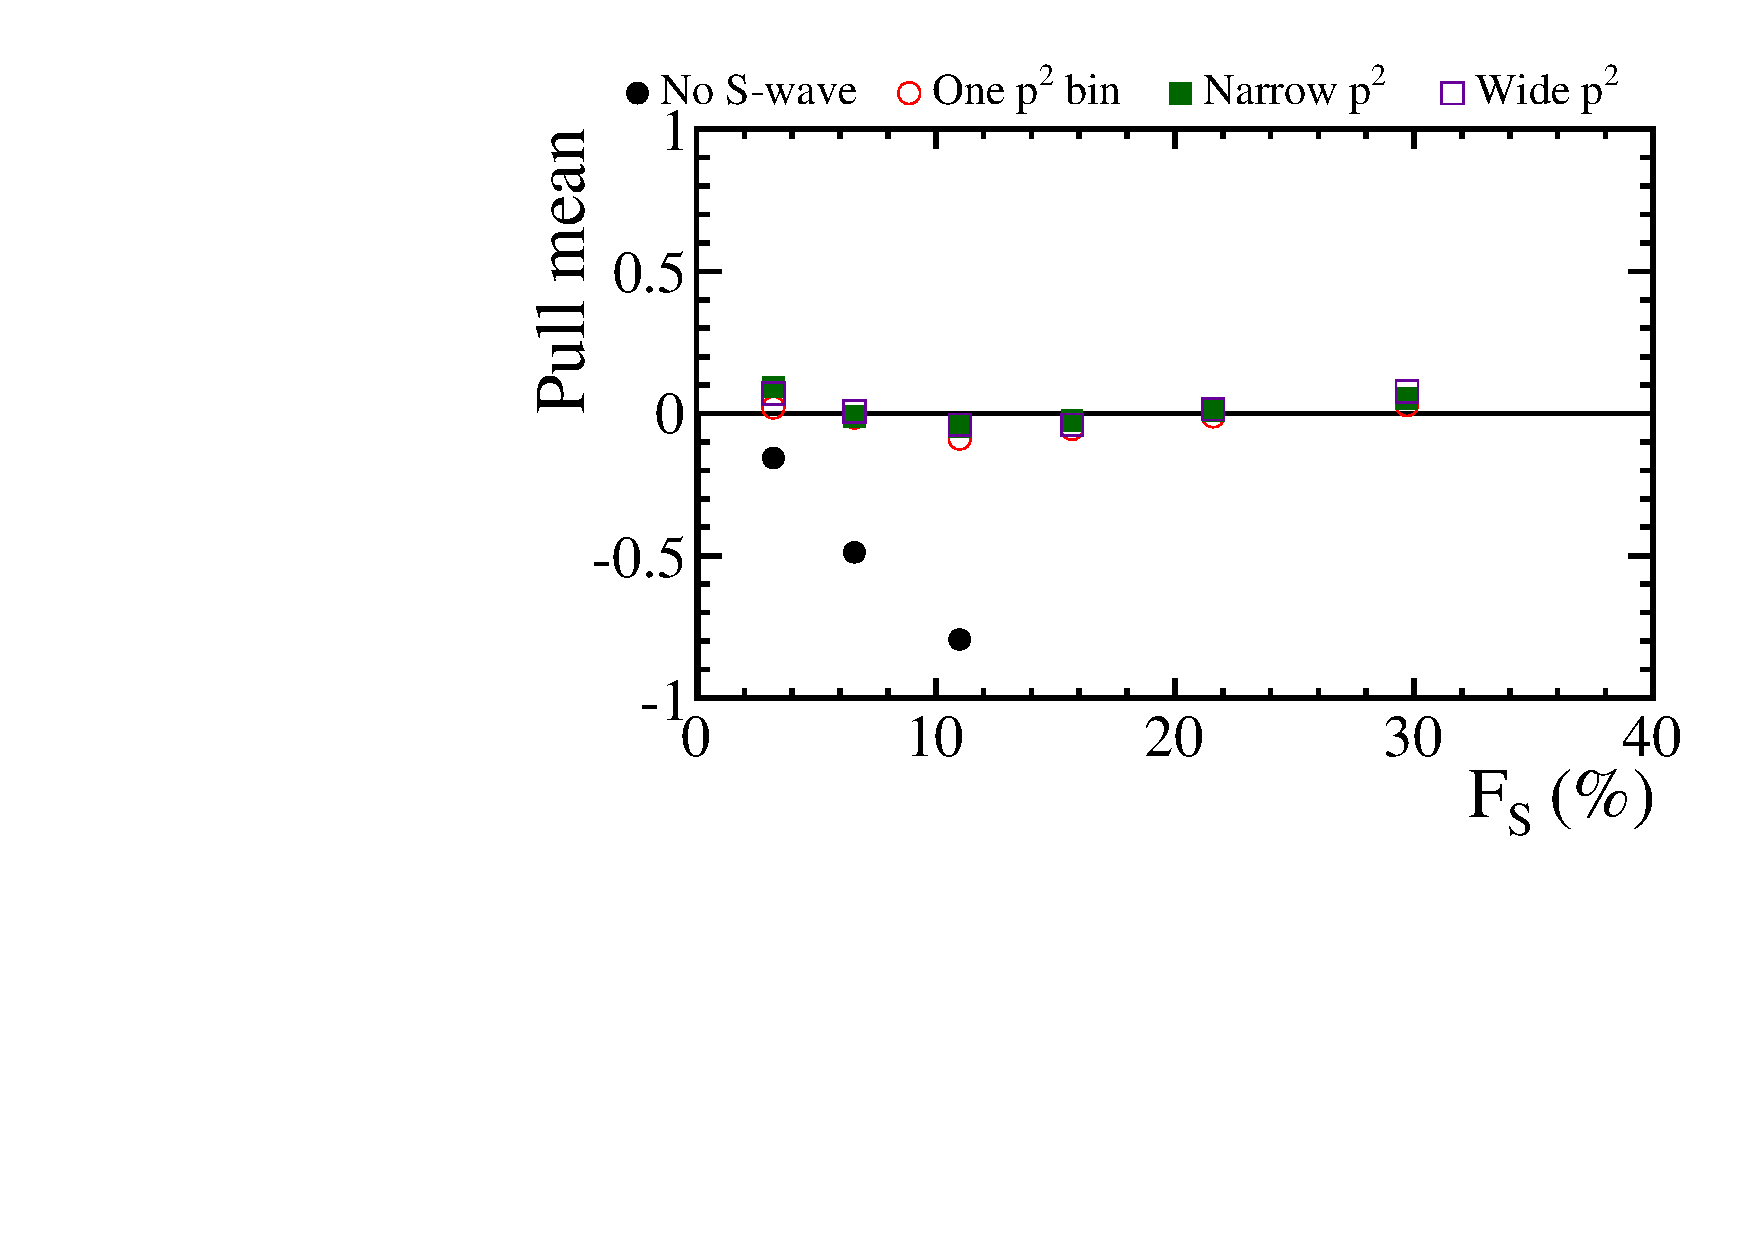
\includegraphics[width=0.48\textwidth]{chapter6/figs/fit_result_combo_fs_fl_mean.pdf}}
\subfigure[\AT2 ]{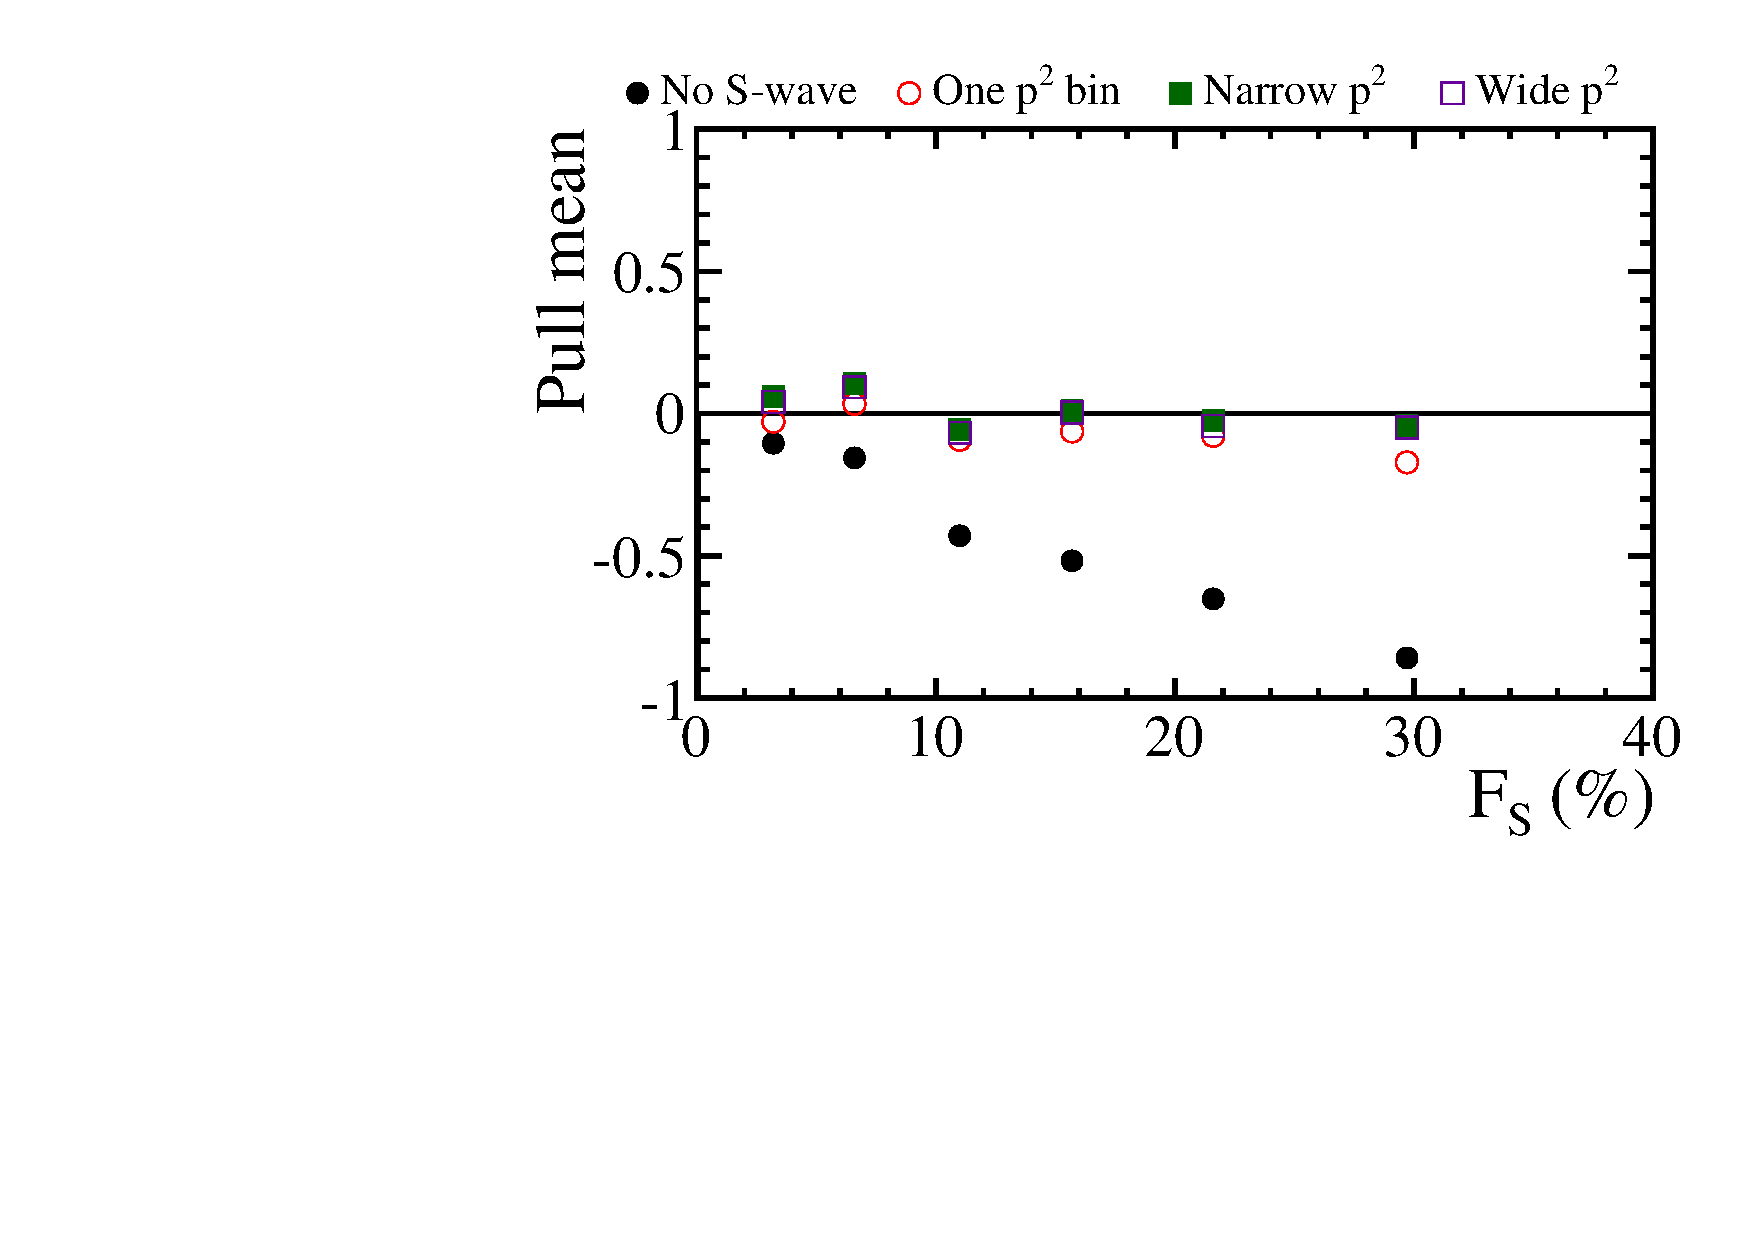
\includegraphics[width=0.48\textwidth]{chapter6/figs/fit_result_combo_fs_at2_mean.pdf}}
\subfigure[\AIm]{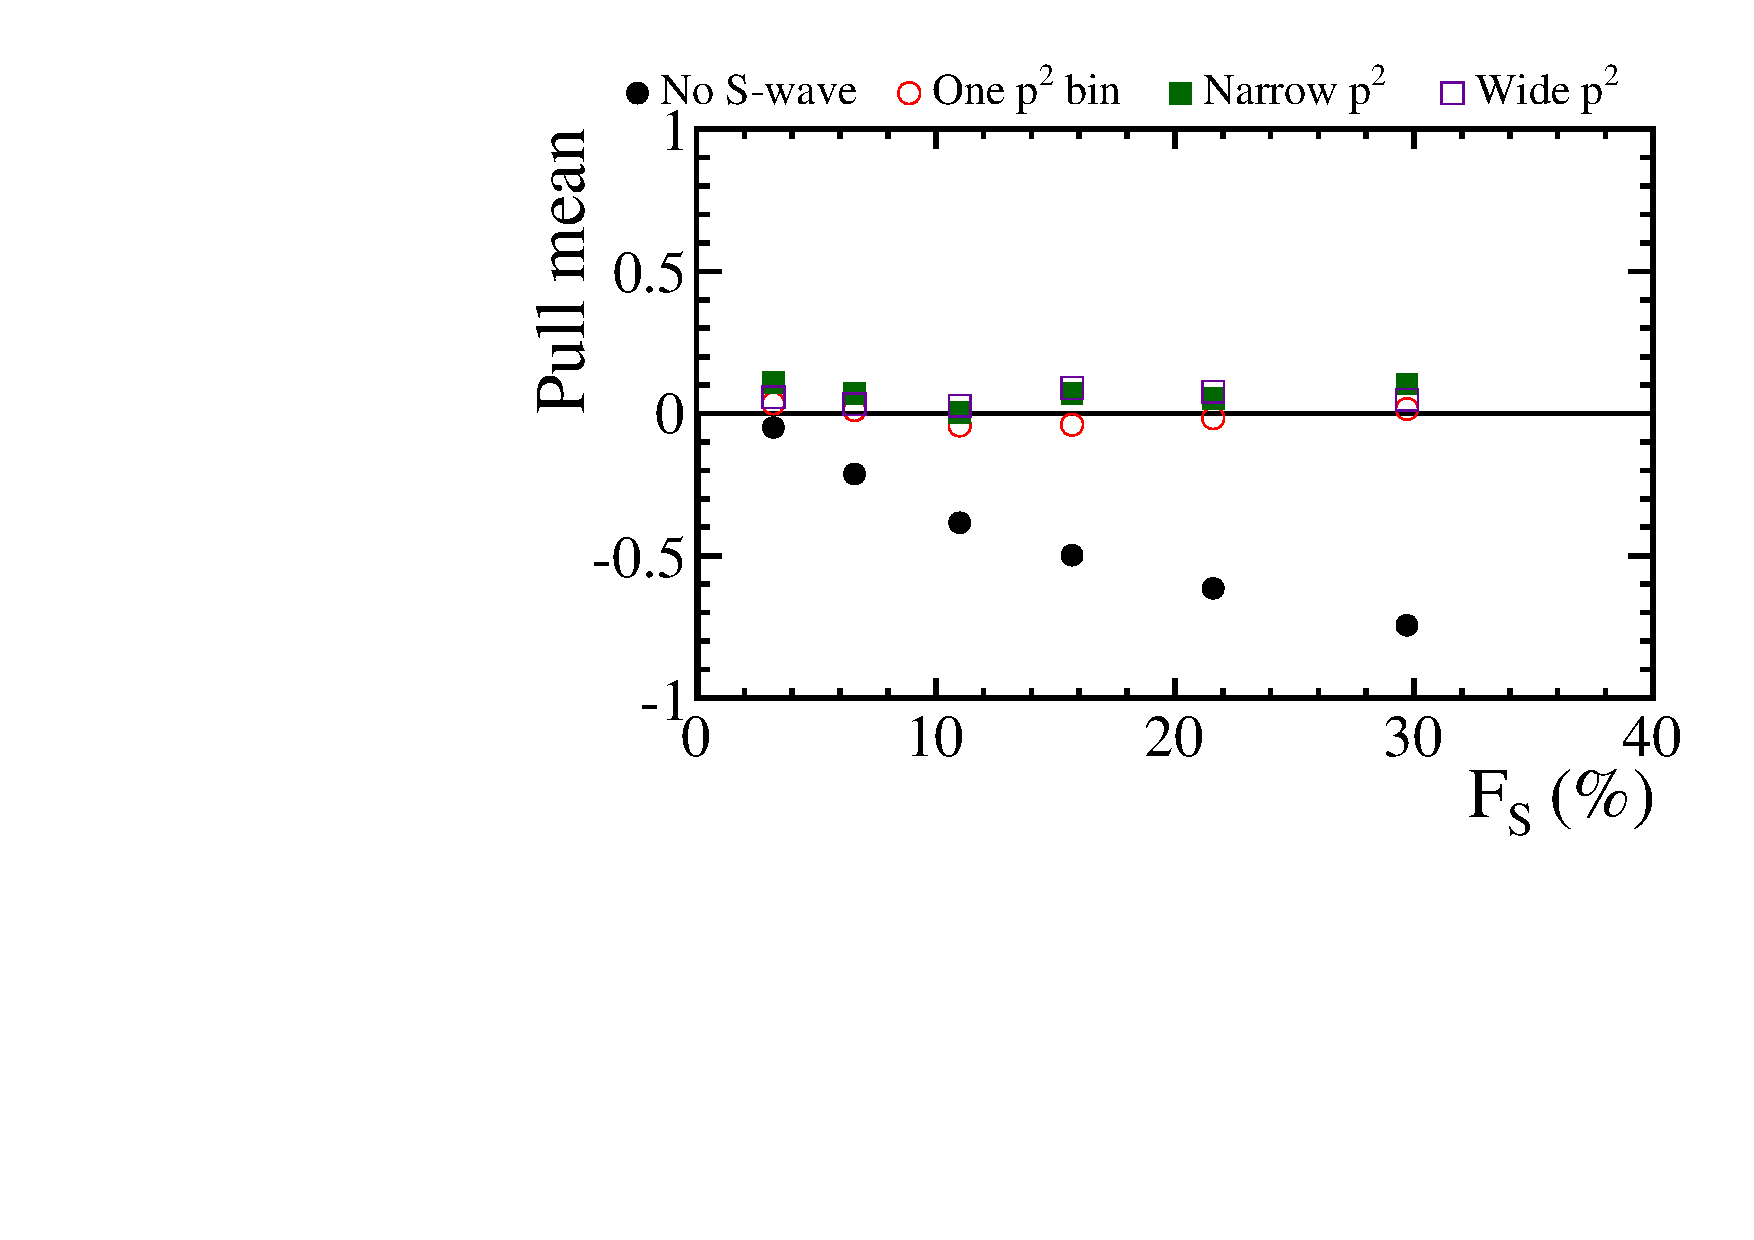
\includegraphics[width=0.48\textwidth]{chapter6/figs/fit_result_combo_fs_aim_mean.pdf}}
\caption[ Pull mean for the three different  
methods to incorporate the S-wave and when the S-wave 
is ignored.    ]
{Pull mean for the three different  
methods to incorporate the S-wave and when the S-wave 
is ignored. There is a slight shift when the S-wave is 
included for datasets of less than 200 events but this is removed from  all the observables 
when the S-wave is included in the fit 
for datasets of over 500 events. ~\label{fig:combofs}}
\end{figure}
The pull width  as a function of S-wave contribution 
for all three fit methods is shown in Fig.~\ref{fig:combofswidth}.
\begin{figure}[tb]
\centering
\subfigure[\AFB]{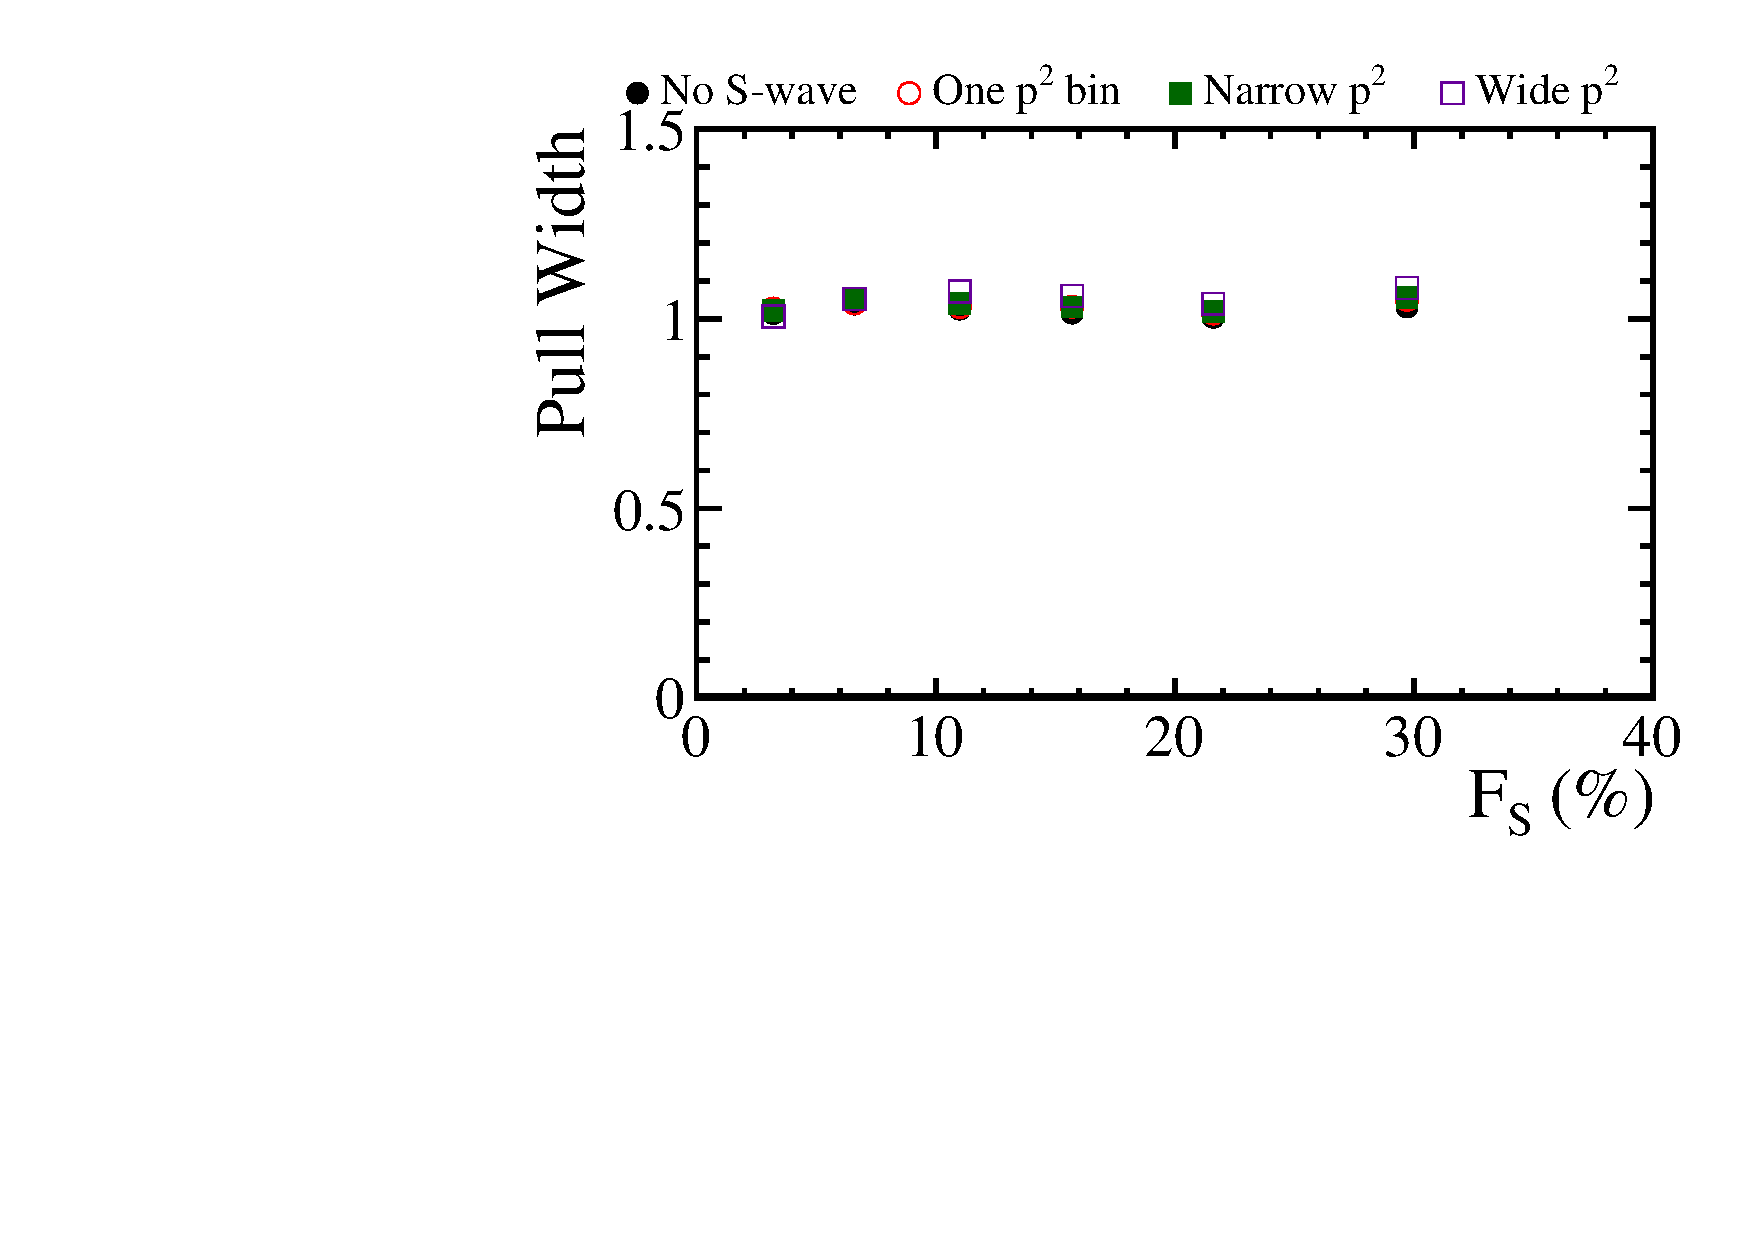
\includegraphics[width=0.48\textwidth]{chapter6/figs/fit_result_combo_fs_afb_width.pdf}}
\subfigure[\FL]{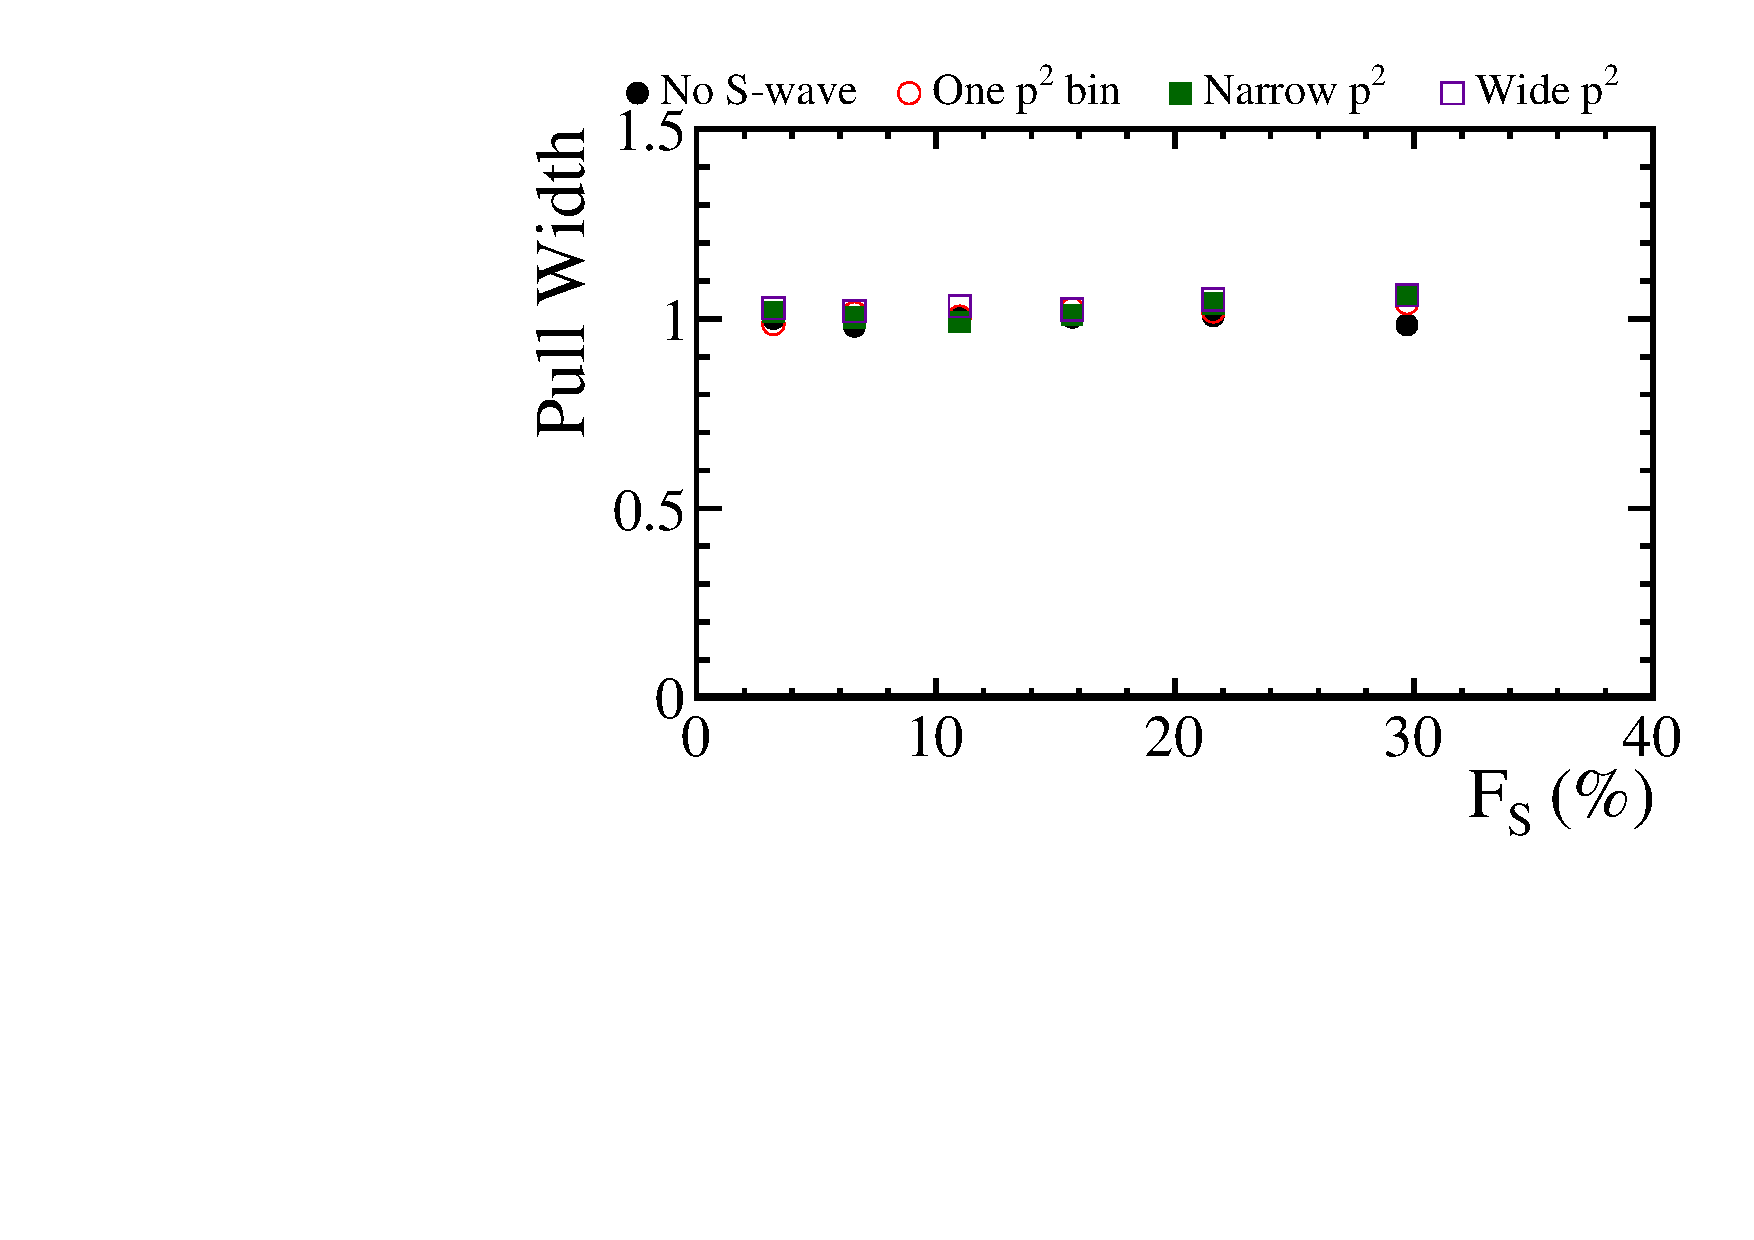
\includegraphics[width=0.48\textwidth]{chapter6/figs/fit_result_combo_fs_fl_width.pdf}}
\subfigure[\AT2 ]{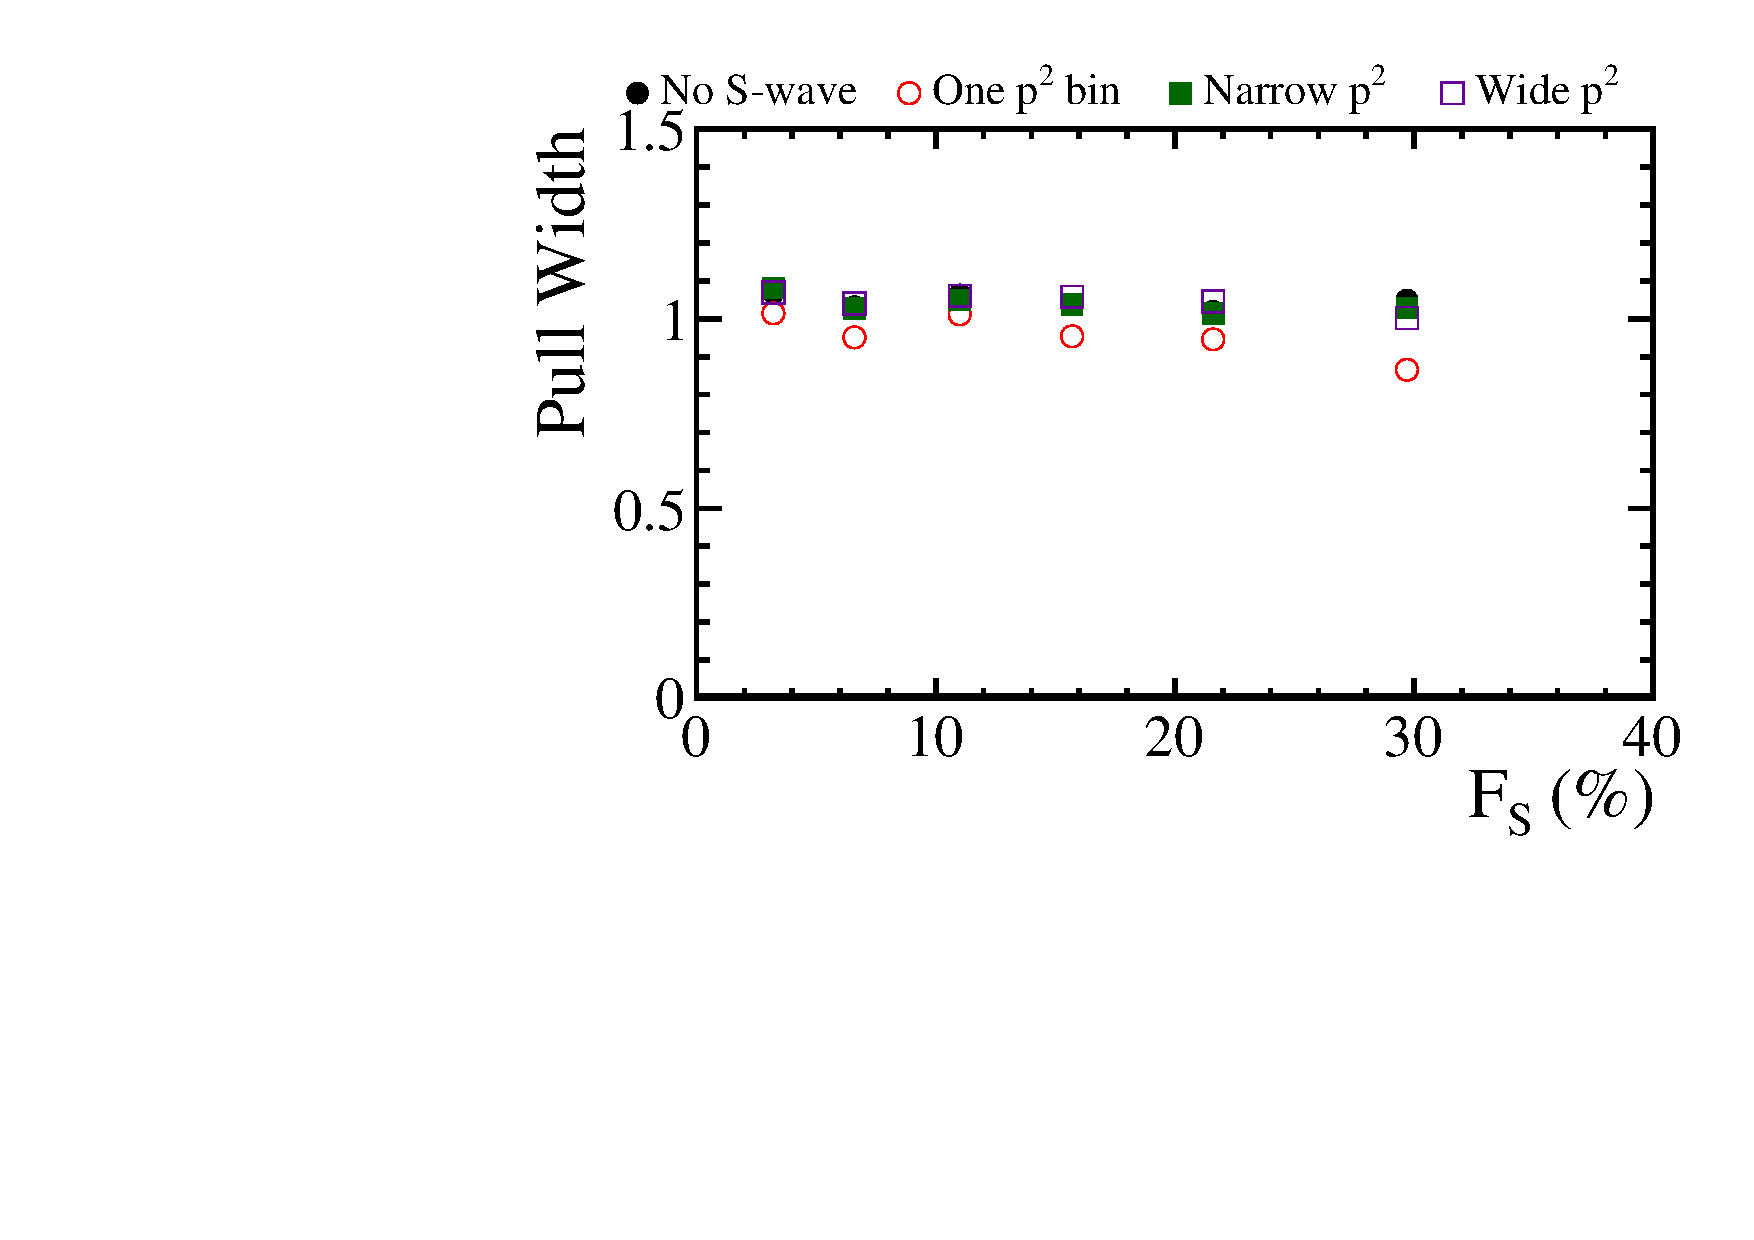
\includegraphics[width=0.48\textwidth]{chapter6/figs/fit_result_combo_fs_at2_width.pdf}}
\subfigure[\AIm]{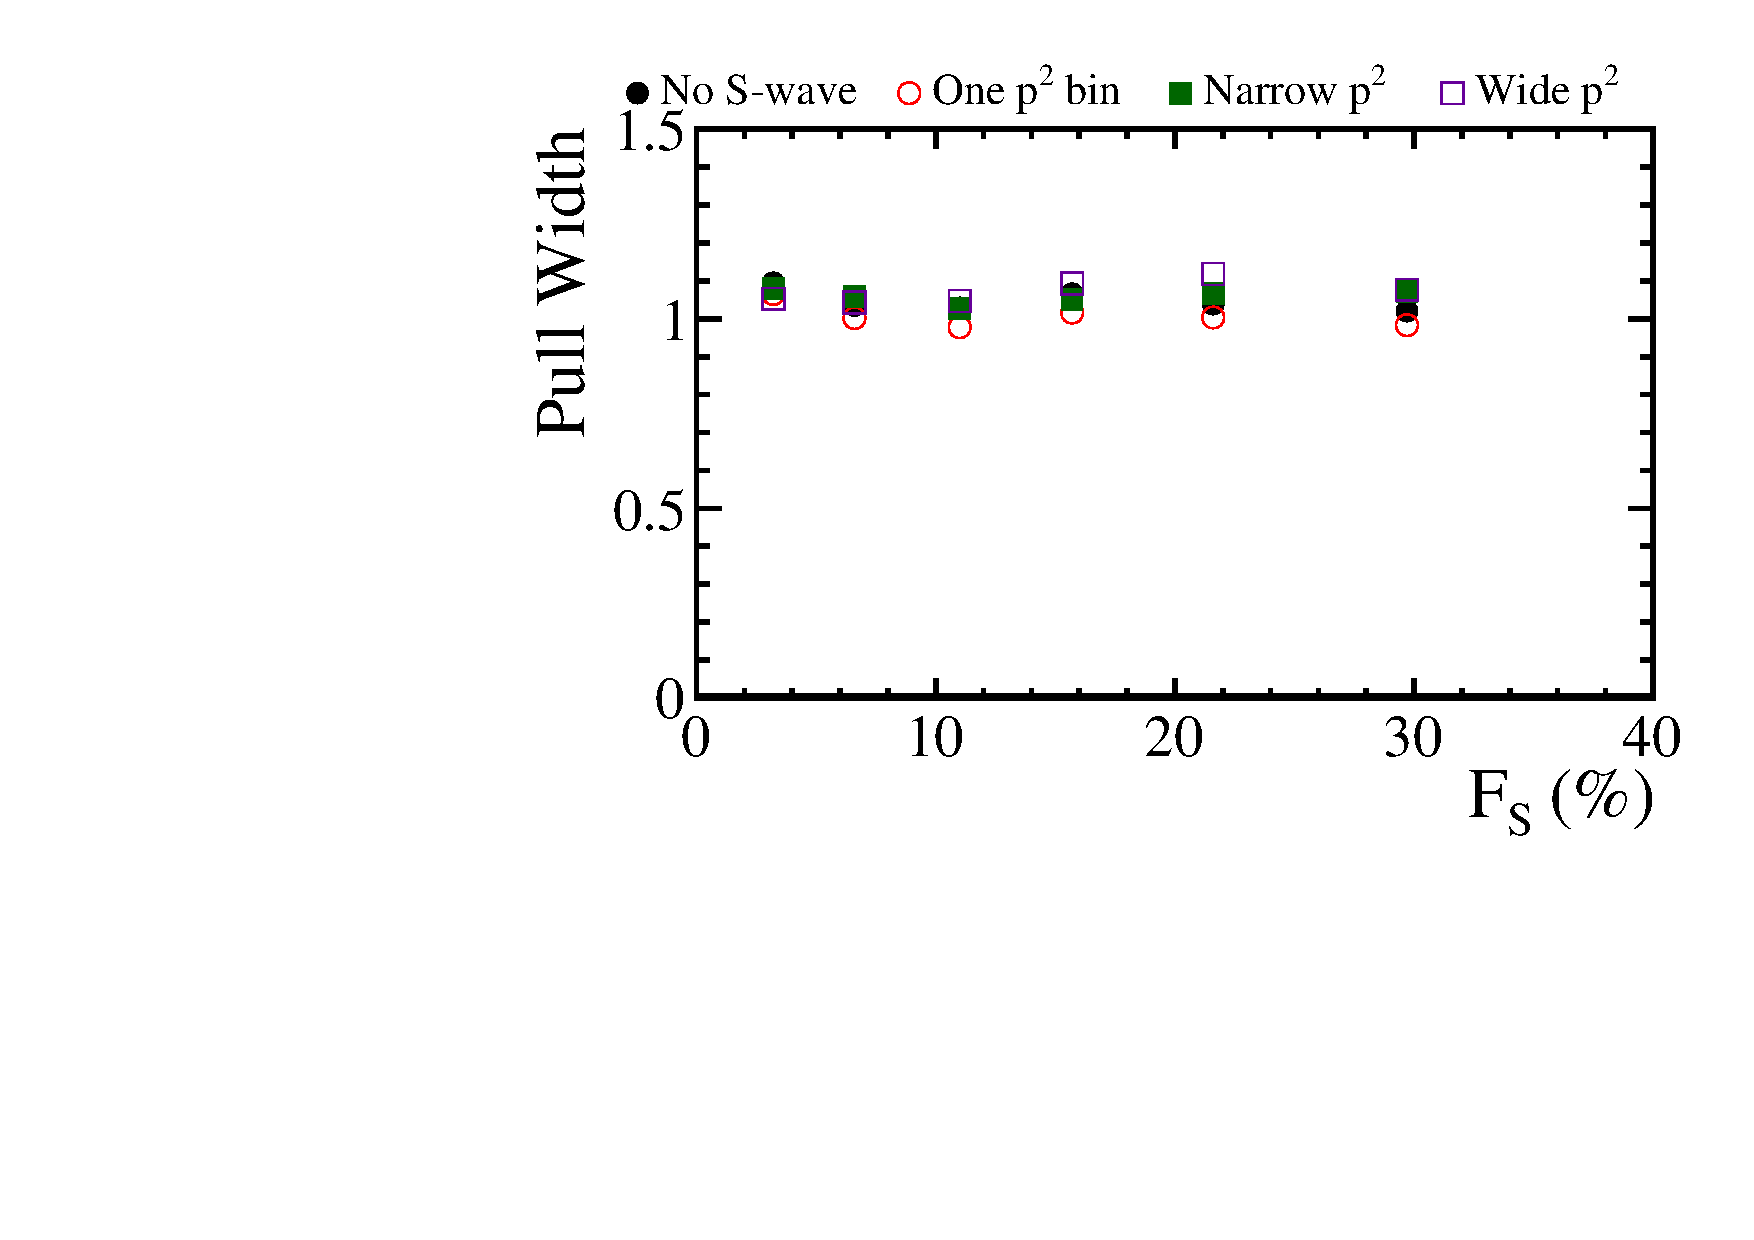
\includegraphics[width=0.48\textwidth]{chapter6/figs/fit_result_combo_fs_aim_width.pdf}}
\caption[ Pull width for the three different  
methods to incorporate the S-wave and when the S-wave 
is ignored.    ]
{Pull width for the three different  
methods to incorporate the S-wave and when the S-wave 
is ignored. There is a slight shift when the S-wave is 
included for datasets of less than 200 events but this is removed from  all the observables 
when the S-wave is included in the fit 
for datasets of over 500 events. ~\label{fig:combofswidth}}
\end{figure}



